% COLING 2027 submission via ACL Rolling Review (deadline 12 October 2026).
% Review version: anonymous, line numbers, page numbers. Switch to \usepackage{acl} for the final version.
%
%
% Working title below. Two alternatives that reflect the new storyline:
%   1. How to Narrow the Label Space for In-Context Classification:
%      Class-Conditional Conformal Prediction Under a Corrected Protocol
%   2. Narrowing the Label Set for In-Context Text Classification:
%      When Conformal Prediction Beats Top-$k$ and When a Classifier Is Enough
\documentclass[11pt]{article}

\usepackage[review]{acl}

\usepackage{times}
\usepackage{latexsym}
\usepackage[T1]{fontenc}
\usepackage[utf8]{inputenc}
\usepackage{microtype}
\usepackage{inconsolata}
\usepackage{graphicx}
\usepackage{booktabs}
\usepackage{amsmath}
\usepackage{multirow}

% Float placement: allow pages that are mostly floats so that the five main-text floats land at the top of the page where they are first cited.
\renewcommand{\topfraction}{0.95}
\renewcommand{\textfraction}{0.05}
\renewcommand{\floatpagefraction}{0.85}
\setcounter{topnumber}{3}
\setcounter{totalnumber}{4}

\title{Evaluating Conformal In-Context Learning Across Tasks and Models}

% Anonymous submission: author block left as in the template.
\author{Anonymous ACL submission}

\begin{document}
\maketitle

% Abstract: at most 150 words (wc -w on the text without comments). Numbers follow paper/figures/NUMBERS.md.
\begin{abstract}
Narrowing the label set before prompting a large language model (LLM) is a cheap aid to in-context text classification.
Conformal In-Context Learning (CICLe) does this with a small classifier calibrated by class-conditional conformal prediction.
Earlier evidence for it came from a protocol with unlisted labels, unequal example pools and unseeded conformal sets, under which up to 65\% of outputs did not parse.
We correct it and evaluate CICLe on five English datasets with eight open LLMs and paired bootstrap tests.
Narrowing gives a small, reliable gain over few-shot prompting, 0.5 to 1.8 macro-F1 points, and 11 to 45\% shorter prompts.
How one narrows matters.
When the labelled pool is long-tailed, class-conditional sets keep their coverage while top-$k$, probability-mass and marginal sets lose 3 to 13 points.
The gain is largest when label names mean nothing.
With 1,600 balanced labels a fine-tuned encoder beats the 3B to 8B pipelines, which win when the pool is skewed or small.
\end{abstract}

\section{Introduction}
\label{sec:intro}

Large language models (LLMs) classify text from a few labelled examples placed in the prompt, without any weight update \citep{brown2020language}.
Which examples are shown, and in what order, can move accuracy by as much as a change in model size \citep{liu2022makes,lu2022fantastically,zhao2021calibrate}, and with many classes the prompt must also carry the label space.

Conformal In-Context Learning (CICLe) was proposed by \citet{randl2024cicle} to make this decision smaller before the LLM sees it.
A small classifier is calibrated with class-conditional conformal prediction so that, for each input, it returns a set of candidate labels that contains the true label with a chosen probability.
The LLM then chooses among these candidates only, with examples retrieved from the candidate classes, and is not called when the set has one element.

CICLe was evaluated on one food-safety dataset.
A pilot study on four further datasets, run with the original CICLe prompts, reported that its benefit grows with class imbalance and that it helps some LLMs and hurts others.
The pilot protocol let only the zero-shot prompt list the admissible labels, drew few-shot and CICLe examples from pools of different size, and left the conformal sets unseeded, so that runs could not be paired.
The first flaw alone made up to 65\% of the outputs of some models unparseable, and the parse failures, not the method, decided which models appeared to benefit.
% ANONYMITY: the pilot is arXiv:2512.05732 by the same authors. Do not cite it. Keep the wording "a pilot study".
This paper replaces the pilot with a corrected protocol and asks a sharper question, namely how a small classifier should narrow the label space for an LLM, and when the LLM is worth calling at all.
We evaluate CICLe on five English datasets, six open LLMs with 3B to 8B parameters and two with 12B and 32B, with three data seeds and paired bootstrap tests over test instances throughout.
Our contributions are the following.
\begin{enumerate}
  \setlength\itemsep{0pt}
  \item \textbf{A corrected protocol.} Every prompt lists the admissible labels, every method retrieves from the same pool, and calibration splits, conformal sets and test samples are seeded. Rerunning the pilot's protocol shows that these choices change conclusions (Section~\ref{sec:res-protocol}).
  \item \textbf{A measured gain.} With wording, pool and seeds held equal, CICLe beats few-shot prompting in nine of ten dataset and retrieval cells by 0.5 to 1.8 macro-F1 points, and shortens Per-Class prompts by 11 to 45\% (Section~\ref{sec:res-gain}).
  \item \textbf{How to narrow.} At equal mean set size, class-conditional conformal sets match top-$k$, probability-mass and marginal conformal sets on balanced data. When the labelled pool is long-tailed, the alternatives lose coverage on the rare classes and 3 to 13 points, which the LLM cannot recover. The gain over few-shot prompting is largest, up to 6.5 points, when label names are nonsense words (Sections~\ref{sec:res-narrowing} and~\ref{sec:res-relabel}).
  \item \textbf{When to call the LLM.} With 1,600 balanced labels, a fine-tuned RoBERTa-base beats every 3B to 8B pipeline on four of five datasets, and on the fifth the base classifier alone does. Under a long-tailed or small pool the order flips. We give a decision rule and a rule for the miscoverage level (Sections~\ref{sec:res-baselines} and~\ref{sec:res-alpha}).
\end{enumerate}
We retract the pilot's imbalance claim. Imbalance widens the gap between narrowing rules, not between CICLe and few-shot prompting.
Code, prompts and per-instance records will be released.
% Anonymised repository placeholder: \url{https://anonymous.4open.science/r/XXXX}

\section{Related Work}
\label{sec:related}

\paragraph{Few-shot prompting and example selection.}
In-context learning lets an LLM classify from labelled examples in the prompt \citep{brown2020language}.
Its accuracy depends on which examples are shown and in what order \citep{lu2022fantastically}, and on biases toward frequent or recent labels that can be corrected after the fact \citep{zhao2021calibrate}.
Retrieving examples that are similar to the test input is the standard remedy \citep{liu2022makes}, either with an off-the-shelf encoder or with a retriever trained for the purpose \citep{rubin2022learning}.
Later work treats selection as a search problem over the labelled pool \citep{purohit2025sampleefficientdemonstrationselection}.
We keep similarity-based retrieval fixed and vary only which classes are allowed to contribute examples.

\paragraph{Two-stage pipelines.}
Pairing a cheap model with an expensive one is an old idea in NLP efficiency.
Cascades send an input to a stronger model only when a weaker one is not confident \citep{varshney2022model,chen2024frugalgpt,yue2024cascades}, and routers learn that decision from data \citep{ding2024hybrid}.
\citet{fisch2021efficient} conformalise such a cascade so that implausible labels are pruned early with a coverage guarantee.
For classification with many labels, a retriever can show the LLM only part of the label space \citep{milios2023incontext}, or the LLM can first generate candidate labels that are then re-ranked \citep{zhu2024icxml,doosterlinck2024incontext}.
CICLe \citep{randl2024cicle} belongs to this family. Its first stage is a supervised classifier whose candidate set is calibrated by conformal prediction, and the LLM is called only when that set has more than one label.
Our comparison of narrowing rules asks which part of this design carries the benefit.

\paragraph{Conformal prediction in NLP and for LLMs.}
Conformal prediction turns any scoring model into a set-valued predictor with a finite-sample coverage guarantee \citep{vovk2005algorithmic,angelopoulos2023gentle}.
Its split (inductive) form needs one held-out calibration set \citep{papadopoulos2002inductive}, and calibrating per class gives coverage that holds within each class rather than on average \citep{vovk2012conditional}.
In NLP it has been applied to classifiers built on pretrained encoders \citep{maltoudoglou2020bert} and, more recently, to LLM outputs: to multiple-choice answers \citep{kumar2023conformal}, to generated text \citep{quach2024conformal}, to models without logit access \citep{su2024api}, and to deciding when an LLM-based agent should ask for help \citep{ren2023robots}.
\citet{campos2024conformal} survey this work.
These methods calibrate the LLM itself. CICLe calibrates a small classifier and uses its sets to shape the LLM's prompt.

\paragraph{Labels in the prompt, and prompting versus fine-tuning.}
Whether the LLM uses the examples or only the label names is contested.
\citet{min2022rethinking} found that random labels barely hurt, and that showing the label space and the input distribution mattered more.
\citet{yoo2022groundtruth} showed that the effect of correct labels depends on the model and the task.
With flipped or semantically unrelated labels, the ability to learn the new mapping grows with model size, and small models fall back on their priors about the label words \citep{wei2023larger,pan2023what,kossen2024incontext}.
Our label renaming experiment uses this setting as a stress test for a narrowing pipeline with 3B to 8B models.
Finally, several evaluations report that a fine-tuned encoder still beats few-shot LLM prompting on standard classification benchmarks when enough labelled data exist \citep{edwards2024language,bucher2024fine,yu2023open,sun2023text}.
We include such a baseline and ask under which data conditions the LLM pipeline pays off.

\section{Background: Narrowing the Label Space with Conformal Prediction}
\label{sec:background}

\paragraph{Split conformal prediction, in plain terms.}
Take any classifier that scores each class.
Hold out a calibration split it has not seen and record, for each calibration example, how low the classifier scored the true label.
For a new input, include in the candidate set every class whose score is no worse than what the true label received on all but a fraction $\alpha$ of the calibration examples.
If the new input is exchangeable with the calibration split, the true label is in the set with probability at least $1-\alpha$, for any classifier and any sample size \citep{vovk2005algorithmic,papadopoulos2002inductive}.
A weak classifier does not lower the coverage, it makes the sets larger.

\paragraph{Class-conditional calibration.}
The guarantee above is marginal over classes.
On a long-tailed dataset the set can cover 95\% of inputs overall while missing most inputs of a rare class, because the rare class contributes few calibration examples to the shared threshold.
Class-conditional conformal prediction computes one threshold per class from the $n_c$ calibration examples of class $c$ only, which guarantees $P(y \in \mathcal{C}(x) \mid y = c) \geq 1-\alpha$ for every class, in expectation over the draw of the calibration split \citep{vovk2012conditional}.
The coverage realised on a finite test sample fluctuates around this level, more so when $n_c$ is small, and with fewer than $1/\alpha - 1$ calibration examples (19 at $\alpha = 0.05$) the class is kept in almost every set.
Top-$k$ selection and probability thresholds give no such guarantee, the first because it ignores the classifier's confidence, the second because it trusts a confidence that is rarely calibrated.

\paragraph{The CICLe pipeline.}
CICLe \citep{randl2024cicle} trains a base classifier (logistic regression on sentence embeddings) on the labelled pool and calibrates it class-conditionally.
For a test input it yields a candidate set $\mathcal{C}(x)$.
If $|\mathcal{C}(x)| = 1$ that label is returned without calling the LLM, and if the set is empty the classifier's top label is.
Otherwise the LLM is prompted with the task description, the candidate labels and labelled examples retrieved from the candidate classes only.

\paragraph{Narrowing rules compared.}\label{sec:rules}
To separate narrowing as such from conformal calibration, we build candidate sets from the same classifier with five rules.
\emph{CP} is the class-conditional conformal set at miscoverage $\alpha$.
\emph{Marginal CP} shares one threshold across classes.
\emph{Top-$m$} keeps the $m$ most probable classes, where $m$ is the mean CP set size on that dataset and seed, so the budget matches but the size does not adapt to the input.
\emph{Probability mass} keeps the most probable classes until their predicted probabilities sum to $1-\alpha$, which adapts but trusts the uncalibrated confidence.
\emph{Oracle} contains the gold label plus $m-1$ random classes and bounds any rule at that size.
All rules share the prompt, the retrieval and the singleton and empty-set behaviour.

\paragraph{Fixed and Per-Class retrieval.}
\emph{Fixed} retrieval places the $k$ training examples most similar to the input (cosine similarity in the embedding space) among those whose label is in the candidate set.
\emph{Per-Class} retrieval places the $k$ most similar examples of each candidate class, so the prompt holds $k \times |\mathcal{C}(x)|$ examples and shrinks with the set.
Few-shot prompting is the case in which the candidate set is the full label set.
Narrowing also makes listing labels affordable, since few-shot prompting must list every class and CICLe only the candidate set.

\section{Experimental Setup}
\label{sec:setup}

\subsection{Datasets}
\label{sec:datasets}

Table~\ref{tab:datasets} lists the six English single-label datasets, chosen to vary the number of classes, the class imbalance, the input length and the information carried by the label names.
SST-5 \citep{socher2013recursive} is the near-balanced five-class case, Yahoo Answers \citep{zhang2015character} has ten balanced topics with informative names and a strong base classifier, SemEval-18 Task~2 \citep{barbieri2018semeval} predicts the emoji of a tweet, so its twenty label names carry little meaning, GoEmotions \citep{demszky2020goemotions}, restricted to single-label comments, is the many-class long-tailed case, and Ohsumed \citep{hersh1994ohsumed} classifies medical abstracts of about 270 tokens into 23 disease categories.
MASSIVE \citep{fitzgerald2023massive} intent classification, with 59 intents of voice-assistant commands of about seven words, adds a second naturally long-tailed dataset with many classes and short inputs from a different domain (Appendix~\ref{app:data}). % PENDING: MASSIVE results arrive over the weekend
The two balanced datasets serve as the substrate for the controlled-imbalance and pool-size experiments, since the skewed ones cannot be rebalanced without changing the task.

% Table 1. Classes and imbalance computed on the training data as loaded (non-empty texts; GoEmotions single-label comments only); mean input length in Llama-3.1 tokens over the seed-42 test sample.
\begin{table}[t]
  \centering
  \small
  \setlength{\tabcolsep}{3.5pt}
  \begin{tabular}{llrrrl}
    \toprule
    \textbf{Dataset} & \textbf{Domain} & \textbf{Cls.} & \textbf{Imb.} & \textbf{Len.} & \textbf{Variants} \\
    \midrule
    SST-5         & Sentiment, reviews &  5 & 2.1$\times$ &  23 & I, P, R \\
    Yahoo Answers & Topic, Q\&A        & 10 & 1.4$\times$ &  50 & I, P, R \\
    SemEval-18    & Emoji, tweets      & 20 & 8.7$\times$ &  20 & R \\
    GoEmotions    & Emotion, Reddit    & 28 & 329$\times$ &  16 & R \\
    Ohsumed       & Disease, abstracts & 23 & 65$\times$  & 271 & R, F \\
    \bottomrule
  \end{tabular}
  \caption{Datasets. \emph{Cls.} is the number of classes, \emph{Imb.} the ratio between the largest and the smallest class in the full training set, \emph{Len.} the mean input length in Llama-3.1 tokens. \emph{Variants}: I = controlled imbalance of the labelled pool (10$\times$, 100$\times$), P = pool size (250, 500, 1,000), R = label renaming, F = Fixed retrieval only beyond $k = 1$ (a Per-Class prompt at $k = 4$ would hold about 90 abstracts). Every dataset is subsampled to 1,600 training, 400 calibration and 1,000 test instances per seed (Section~\ref{sec:protocol}).}
  \label{tab:datasets}
\end{table}


\subsection{Models}
\label{sec:models}

The main grid uses six open instruction-tuned LLMs, two sizes from each of three families: Llama-3.2-3B and Llama-3.1-8B \citep{grattafiori2024llama3}, Qwen2.5-3B and Qwen2.5-7B \citep{qwen2024qwen25}, Ministral-3-3B \citep{mistral2025ministral3} and Mistral-7B-v0.3 \citep{jiang2023mistral7b}. % CHECK that the Llama 3 herd report is the right citation for Llama-3.2-3B
Mistral-NeMo-12B \citep{mistralai2024nemo} and Qwen2.5-32B \citep{qwen2024qwen25} are run with and without CICLe on the five short-text datasets (Appendix~\ref{app:large}). % PENDING: 12B and 32B on Ohsumed and MASSIVE
All run in bfloat16 with greedy decoding through their chat templates.
The base classifier of every narrowing method is logistic regression on \texttt{all-MiniLM-L6-v2} sentence embeddings \citep{reimers2019sentence,wang2020minilm}, and the same embeddings retrieve the examples by cosine similarity, so MiniLM is both the classifier's feature space and the retriever.
Calibration uses \texttt{crepes} \citep{bostrom2022crepes} with seeded tie-breaking.
Contriever \citep{izacard2022unsupervised}, TF-IDF and an SVM appear in the ablations.

\subsection{Protocol}
\label{sec:protocol}

Every experiment uses a stratified subsample of 2,000 labelled and 1,000 test instances per dataset, drawn with three seeds (42, 43, 44).
Of the 2,000, 400 form the calibration split, the proportion of \citet{randl2024cicle}, and the base classifier, the retrieval pool and the supervised baselines all see the same 1,600 training examples.
One test sample per seed is shared by every method, which makes paired tests over instances possible, and the seeds change the subsample, the calibration split and the conformal tie-breaking (Appendix~\ref{app:prompt} gives the reasoning behind the sizes).

\paragraph{Holding the label information constant.}
The released CICLe implementation lists no labels in its prompt, which suits its Per-Class retrieval because every candidate class appears among the examples, and saves context when there are hundreds of classes.
Our comparison adds Fixed retrieval and zero-shot and few-shot prompting, whose prompts show few or no labels, so every prompt lists the admissible labels, all classes or the candidate set.
Without this, prompts that show only the retrieved labels left up to 65\% of a model's outputs unparseable and changed the sign of the per-model effect of narrowing in a third of the cells (Appendix~\ref{app:original}). % PENDING: label-list ablation (only the list removed, same parser and token budget; every dataset, seed 42, Fixed and Per-Class, k in {1,4}) will replace the original-format comparison as the evidence and separate the list from the parser and the 5-token cap
Every method also retrieves from the same pool, the calibration split, conformal sets and test sample are seeded, outputs are normalised before matching, and an output that matches no label counts as wrong (Appendix~\ref{app:prompt}).

Both retrieval variants are run for every prompting method, with $k \in \{1, 2, 4, 8\}$ on the five short-text datasets and $k \in \{1, 4\}$ elsewhere, and Per-Class retrieval on Ohsumed at $k = 1$ only (Appendix~\ref{app:prompt}).
The reference setting is MiniLM, logistic regression and $\alpha = 0.05$, the choices of the original paper.

\subsection{Experiments}
\label{sec:experiments}

Each experiment beyond the main grid isolates one variable.
\emph{Narrowing rules}: the four alternative rules of Section~\ref{sec:rules} on every dataset and variant, $k \in \{1, 4\}$. Top-$m$ is matched to CICLe's mean set size. % PENDING: size-matched probability-mass and marginal rules
\emph{Controlled imbalance}: on SST-5 and Yahoo Answers the training sample is replaced by a long-tailed one whose class sizes decay geometrically to a ratio of 10 or 100, with at least five examples per class and a class order drawn from the seed, while the test sample is unchanged (Appendix~\ref{app:data}).
\emph{Label renaming}: on all six datasets every class name is replaced by a nonsense word, the same for all seeds, leaving texts, splits and classifier unchanged.
\emph{No examples}: CICLe with $k = 0$ shows the candidate list alone.
\emph{Pool size}: on SST-5 and Yahoo Answers the labelled pool is reduced to 250, 500 and 1,000 examples, split 80/20 as before, with every pipeline and baseline rerun.
\emph{Ablations}: $\alpha \in \{0.01, 0.05, 0.10, 0.20\}$, the embedding and the classifier, with Llama-3.1-8B and Llama-3.2-3B on the short-text datasets. % PENDING: Ohsumed, MASSIVE and the remaining models for the SVM and embedding ablations
\emph{Prompt robustness}: a second template with the labels in random order and the most similar example last, and random instead of similarity-based retrieval, on seed 42 with $k \in \{1, 4\}$. % PENDING: random retrieval on SST-5, SemEval-18 and Ohsumed

\paragraph{Roadmap.}
Section~\ref{sec:res-coverage} measures per-class coverage, Section~\ref{sec:res-narrowing} compares the rules at matched set size under controlled and natural imbalance, Section~\ref{sec:res-consequence} pairs instances to see what a missing label costs, Section~\ref{sec:res-gain} uses the main grid, $k = 0$ and label renaming to show when narrowing pays off, and Section~\ref{sec:res-secondary} covers the baselines, pool sizes, $\alpha$ and larger models.

\subsection{Methods and Baselines}
\label{sec:methods}

\emph{Zero-shot} prompting lists all labels and no examples, \emph{few-shot} prompting adds retrieved examples from all classes, and \emph{CICLe} restricts both to the class-conditional conformal set, returning a singleton set without an LLM call and the classifier's top label for an empty set.
The alternative narrowing rules differ from CICLe only in the set.
Three supervised baselines use no LLM, namely the base classifier itself, and RoBERTa-base and RoBERTa-large \citep{liu2019roberta} fine-tuned on the same 1,600 examples for ten epochs (AdamW, learning rate $2 \times 10^{-5}$ for base and $10^{-5}$ for large, batch size 16, 256 tokens, linear warm-up and decay) with the epoch chosen on the 400 calibration examples.
The recipe is not tuned further, so the encoder scores are a floor. All baselines are run for three seeds and every dataset variant.

\subsection{Metrics and Statistics}
\label{sec:metrics}

We report macro-F1 over the classes present in the test sample (accuracy is in Appendix~\ref{app:full}), the invalid-output rate, the expected input tokens per test instance with no-call instances counted as zero, and the overall, class-averaged and lowest per-class coverage and mean size of the candidate sets. % PENDING: expected tokens per instance and class-averaged coverage in the tables
Every comparison between two methods is paired, with both sharing the model, seed, $k$ and retrieval variant, hence the same test instances, pool and conformal sets.
We report the mean paired macro-F1 difference over all such cells with a 95\% interval from a bootstrap with 5,000 resamples of the test instances \citep{koehn2004statistical,dror2018hitchhiker}, with the same resample applied to both methods in every cell, so the interval reflects test-sample noise and not the spread over hyperparameters.
The number of pairs is 72 for the main grid (six models, three seeds, four values of $k$), 36 where $k \in \{1, 4\}$, 12 or 6 per model and 12 for the seed-42 checks.
For the main deltas we also report a hierarchical bootstrap that resamples models, seeds and instances, and the number of (model, seed) cells with a positive sign. A difference is significant when its interval excludes zero, printed in bold in the tables, otherwise marked n.s. % PENDING: hierarchical intervals and sign counts

\section{Results}
\label{sec:results}

% SKELETON. Prose is drafted in paper/plan/results_section_draft.md and will be inserted when the
% pending runs (Ohsumed PC k=1, marginal CP, k=0, oracle, pool size, 32B seeds) are in.
% Every subsection opens with its claim, then the float, then the numbers (see STYLE_NOTES.md).
% All numbers at the reference setting (MiniLM, logistic regression, alpha = 0.05), six models x three seeds.

\subsection{The Protocol Decides the Conclusion}
\label{sec:res-protocol}
% CLAIM: Listing the labels, sharing the pool and seeding the sets reverse the pilot's model-level picture;
% invalid outputs fall to 0-6% and no model is significantly hurt by Per-Class CICLe (Appendix D, G).

\subsection{Narrowing the Label Set Helps a Little, and Reliably}
\label{sec:res-gain}
% CLAIM: CICLe beats few-shot in 8 of 9 dataset x variant cells by +0.5 to +1.8 points (72 pairs) and
% Per-Class CICLe uses 11-38% fewer prompt tokens at equal k; the gain does not vanish at k=8.
% Table 2 (full width): main results at k = 4 plus paired deltas over all k. Spec: figures_and_tables.md.
% PLACEHOLDER until analyze.py --bootstrap 5000 has been rerun.
\begin{table*}[t]
  \centering
  \small
  % TODO: rows MiniLM+LR, RoBERTa, zero-shot, few-shot Fixed, CICLe Fixed, few-shot PC, CICLe PC (k=4, mean prompt tokens in small type),
  %       then Delta Fixed and Delta PC over all k with 95% CI; columns Yahoo | SST-5 | SemEval-18 | GoEmotions | Ohsumed.
  \begin{tabular}{lccccc}
    \toprule
    & Yahoo & SST-5 & SemEval-18 & GoEmotions & Ohsumed \\
    \midrule
    \multicolumn{6}{c}{\emph{placeholder}} \\
    \bottomrule
  \end{tabular}
  \caption{Macro-F1 at $k = 4$ for every method (mean over six models and three seeds, supervised rows over three seeds), with the mean prompt tokens per LLM call in small type, and the paired difference CICLe minus few-shot pooled over all $k$ with its 95\% bootstrap interval. Same prompt wording, same 1,600-example pool, seeded conformal sets, paired bootstrap over test instances. Bold marks intervals that exclude zero.}
  \label{tab:main}
\end{table*}

% Figure 1 (full width). Generated by make_figures.py (fig1).
\begin{figure*}[t]
  \centering
  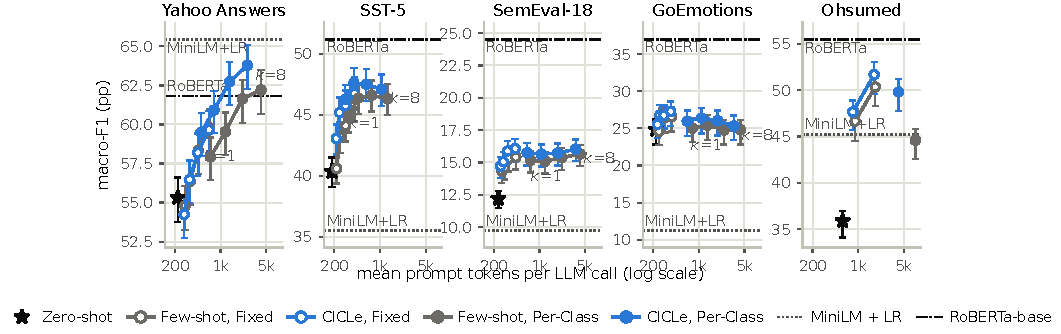
\includegraphics[width=\textwidth]{figures/f1_vs_tokens.pdf}
  \caption{Macro-F1 against mean prompt tokens per LLM call (log scale), one panel per dataset. Every point is one (method, retrieval variant, $k$) at the reference setting, averaged over six models and three seeds, with $k$ increasing along each line. Hollow markers: Fixed retrieval. Filled: Per-Class. Grey: few-shot. Blue: CICLe. Star: zero-shot. Dotted and dash-dot lines: MiniLM with logistic regression and fine-tuned RoBERTa-base (three-seed means). Error bars are 95\% bootstrap intervals of the 18-run mean over test instances, not the spread over hyperparameters. Ohsumed Per-Class is $k = 1$ only.}
  \label{fig:tokens}
\end{figure*}


\subsection{How You Narrow Matters}
\label{sec:res-narrowing}
% CLAIM: At equal mean set size CP = top-k = mass on balanced data; under a long-tailed labelled pool the
% alternatives lose coverage on rare classes and 4-11 macro-F1 points. Imbalance does NOT widen the
% CICLe-vs-few-shot gap (explicit retraction of the pilot's claim). Coverage bounds the damage (fixes vs breaks).
% Appendix figure (text width): fig_app_narrowing_extra.pdf, the panels of the narrowing analysis not shown in Figure 2.
\begin{figure*}[t]
  \centering
  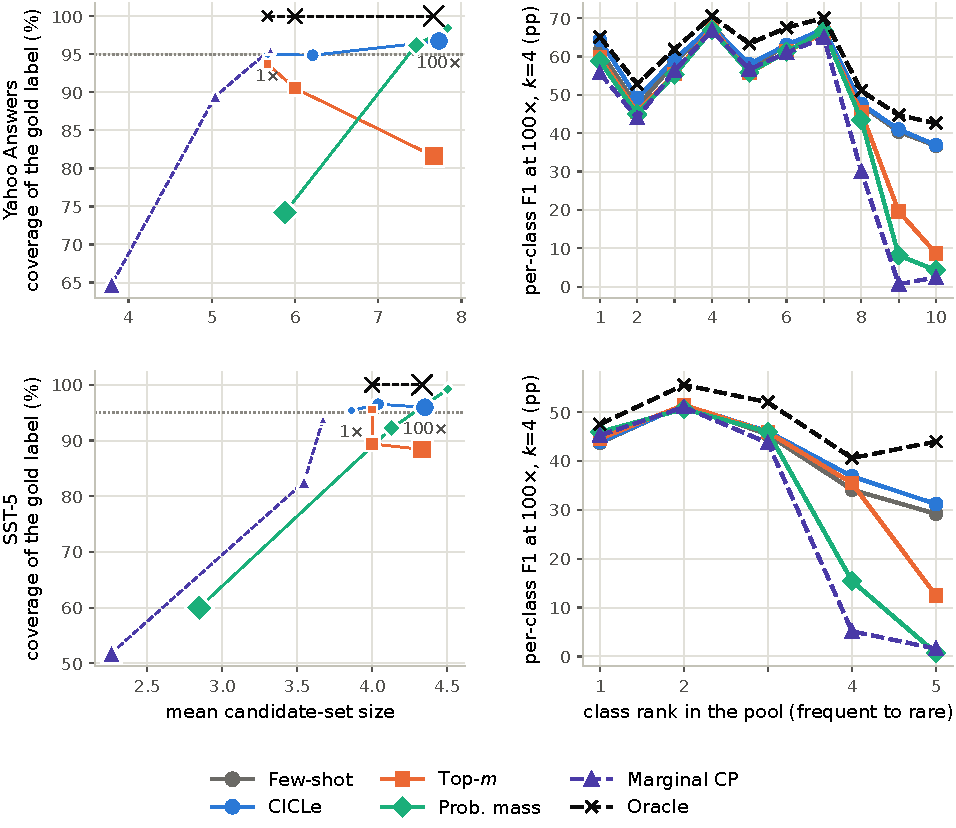
\includegraphics[width=\textwidth]{figures/fig_app_narrowing_extra.pdf}
  \caption{Further panels of the narrowing analysis (Per-Class retrieval, rows Yahoo Answers and SST-5). Left: coverage of the gold label against mean candidate-set size for every rule at 1, 10 and 100 times imbalance (marker size grows with imbalance), mean over three seeds, with the $1 - \alpha$ target dotted. Right: per-class F1 at 100 times imbalance and $k = 4$ by class-frequency rank in the pool, mean over six models and three seeds.}
  \label{fig:imbalance}
\end{figure*}


\subsection{Uninformative Label Names}
\label{sec:res-relabel}
% CLAIM: With every label renamed to a nonsense word, CICLe's margin over few-shot is the largest measured
% (+6.5 Fixed / +5.6 PC on Yahoo; +0.7 / +1.0 on GoEmotions, 36 pairs).
% Table 3 (column width): original vs renamed labels. Spec: figures_and_tables.md. PLACEHOLDER.
\begin{table}[t]
  \centering
  \small
  % TODO: Dataset | Labels | k | Few-shot Fixed | CICLe Fixed | Few-shot PC | CICLe PC; Yahoo and GoEmotions, k in {1,4}; final row paired delta on renamed labels (36 pairs).
  \begin{tabular}{llrrrrr}
    \toprule
    Dataset & Labels & $k$ & FS-F & CICLe-F & FS-PC & CICLe-PC \\
    \midrule
    \multicolumn{7}{c}{\emph{placeholder}} \\
    \bottomrule
  \end{tabular}
  \caption{Macro-F1 with the original label names and with every class renamed to a nonsense word (same mapping for all seeds). The base classifier is unaffected, so the whole effect is on the LLM's use of the candidate list. FS: few-shot. F: Fixed. PC: Per-Class.}
  \label{tab:relabel}
\end{table}


\subsection{When the LLM Pipeline Is Worth It}
\label{sec:res-baselines}
% CLAIM: With 1,600 balanced labels fine-tuned RoBERTa-base beats every pipeline on 4 of 5 datasets and the
% base classifier alone wins on Yahoo; at 100x imbalance the order flips. [PENDING pool size.] Decision rule.
% Table 4 (appendix, full width). Body generated by make_figures.py (tab4).
\begin{table*}[t]
  \centering
  \scriptsize
  \setlength{\tabcolsep}{3pt}
  % Table 4. Macro-F1; supervised rows mean over 3 seeds, LLM rows over 6 models x 3 seeds. Zero-shot does not depend on the pool (1x column only). F = Fixed retrieval (Ohsumed has no Per-Class runs). Bold = best per column.
\begin{tabular}{lccccccccc}
\toprule
 & Yahoo Answers 1$\times$ & Yahoo Answers 10$\times$ & Yahoo Answers 100$\times$ & SST-5 1$\times$ & SST-5 10$\times$ & SST-5 100$\times$ & SemEval-18 & GoEmotions & Ohsumed \\
\midrule
MiniLM + LR & \textbf{65.4} & 50.4 & 31.4 & 35.5 & 20.5 & 12.6 & 9.7 & 11.2 & 45.2 \\
RoBERTa-base, fine-tuned & 61.8 & 58.7 & 41.2 & \textbf{51.2} & 44.5 & 31.9 & \textbf{24.5} & \textbf{37.0} & 55.4 \\
RoBERTa-large, fine-tuned & 64.6 & \textbf{61.6} & 44.9 & 39.9 & 35.8 & 32.2 & 23.0 & 27.3 & \textbf{66.1} \\
Zero-shot & 55.3 & -- & -- & 40.3 & -- & -- & 12.2 & 24.9 & 35.9 \\
Few-shot PC, $k$=4 & 61.6 & 59.4 & 54.6 & 46.6 & 44.6 & 40.8 & 15.4 & 24.8 & 50.4\textsuperscript{F} \\
CICLe PC, $k$=4 & 62.7 & 60.3 & 55.4 & 47.5 & \textbf{46.5} & 41.9 & 15.7 & 26.0 & 51.7\textsuperscript{F} \\
Best LLM pipeline & 63.8 {\scriptsize CICLe PC $k$=8} & 60.3 {\scriptsize CICLe PC $k$=4} & \textbf{56.0} {\scriptsize CICLe PC $k$=1} & 47.6 {\scriptsize CICLe PC $k$=2} & \textbf{46.5} {\scriptsize CICLe PC $k$=4} & \textbf{43.4} {\scriptsize CICLe PC $k$=1} & 16.1 {\scriptsize CICLe F $k$=8} & 27.3 {\scriptsize CICLe F $k$=8} & 53.1 {\scriptsize CICLe F $k$=8} \\
\bottomrule
\end{tabular}

  \caption{Supervised baselines against LLM pipelines, macro-F1. Supervised rows are means over three seeds, LLM rows over six models and three seeds. The fixed configuration is Per-Class retrieval at $k = 4$ (Ohsumed: Fixed, marked F). The best pipeline is the best (method, variant, $k$) mean per column and is selected on the test set. Zero-shot prompting does not depend on the pool. The test sample is identical at every imbalance level. Bold marks the best value per column.}
  \label{tab:baselines}
\end{table*}


\subsection{Choosing $\alpha$, and Robustness Across Models}
\label{sec:res-alpha}
% CLAIM: A looser alpha pays where the classifier is strong (Yahoo) or sets are otherwise huge (GoEmotions),
% is flat on SST; embedding matters more than classifier; no model is hurt by PC CICLe; 12B and 32B models
% also gain (Appendix F); a 3B model with CICLe PC matches 32B zero-shot on the same seed.
% Figure 3 (column width, two stacked panels): choosing alpha. Spec: figures_and_tables.md. PLACEHOLDER.
% Candidate for the appendix if the page budget bites (presentation_plan.md, resolution (a)).
\begin{figure}[t]
  \centering
  % 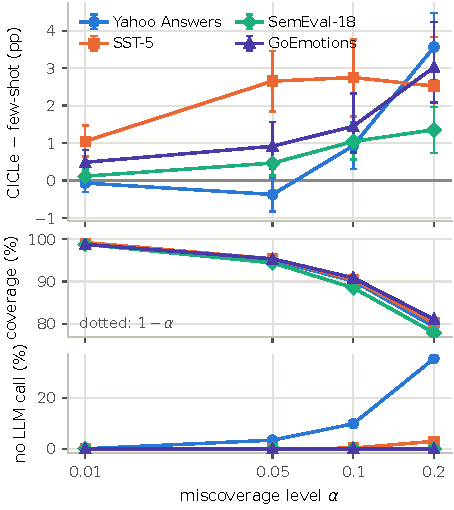
\includegraphics[width=\columnwidth]{figures/alpha.pdf}
  \fbox{\parbox{0.95\columnwidth}{\centering\vspace{3em}\emph{Figure 3 placeholder: $\Delta$ vs.\ few-shot and LLM-skip rate against $\alpha$}\vspace{3em}}}
  \caption{Effect of the miscoverage level $\alpha$. Top: paired difference CICLe minus few-shot, one line per dataset (Llama-3.1-8B and Llama-3.2-3B, 24 cells). Bottom: share of test instances answered by the base classifier alone. Annotations give the empirical coverage at each $\alpha$.}
  \label{fig:alpha}
\end{figure}


\section{Conclusion}
\label{sec:conclusion}

Overall coverage hides unreachable classes. A narrowing rule can contain the gold label for almost every test instance and still never offer a rare class. Rule: inspect per-class coverage, not overall coverage, before trusting a narrowing rule.

At matched set size the narrowing rule matters under a skewed labelled pool and not on balanced data, and under a 100-fold skew the wrong rule costs several times what narrowing gains over few-shot prompting. Rule: calibrate per class whenever the labelled pool is skewed.

The LLM almost never recovers a label that is missing from the candidate set, so the set is a hard constraint. Rule: choose $\alpha$ with the rare classes in mind, since their coverage bounds macro-F1.

Narrowing pays off modestly on short texts with informative labels and more when label names carry no meaning, and for the encoder recipes we tested, fine-tuning wins on a plentiful balanced pool. Rule: prompt with a class-conditionally narrowed list when labels are skewed or scarce, and fine-tune when they are plentiful and balanced.

\section*{Limitations}
\label{sec:limitations}

% SKELETON. One plain paragraph, each item one or two sentences with its consequence (see STYLE_NOTES.md).
% Content from presentation_plan.md:
% - Single-label classification only; GoEmotions restricted to single-label comments. Multi-label narrowing
%   would need a different set construction (R1).
% - 1,000-instance test samples per seed; intervals are correspondingly wide for per-model comparisons
%   (12 or 6 pairs).
% - Six open models of 3-8B parameters; 12B and 32B only partially (32B one seed [PENDING]); no proprietary
%   models; no 70B under the fixed protocol.
% - English only.
% - alpha is chosen on calibration coverage, not tuned; the alpha ablation uses two models.
% - The CP guarantee is marginal within each class, not conditional on the input; coverage can still vary
%   across inputs within a class.
% - Label renaming is an extreme stress test; real deployments sit between informative and nonsense names.
% - Controlled imbalance on two datasets only; naturally skewed datasets confound imbalance with other properties.
% - Bootstrap intervals quantify test-sample noise only, with hyperparameters fixed at the reference setting.


% No acknowledgements in the review version.

\bibliography{references}

\appendix
% Appendix. Unlimited length. Table bodies are generated by paper/figures/make_figures.py and copied
% into tables/body_*.tex; captions and lead sentences live here and in the wrapper files.

\section{Protocol Details, Prompt Template and Output Parsing}
\label{app:prompt}

\paragraph{Why these sizes.}
Two thousand labelled examples per dataset are enough for a usable base classifier on 5 to 28 classes and few enough that every configuration runs for six models and three seeds, at about one GPU-minute per Fixed configuration and up to 17 for Per-Class retrieval at $k = 8$ on a 24\,GB GPU. The 400-example calibration split is the 20\% of the original CICLe paper. The 1,000-instance test sample is shared by every method on a seed, and its bootstrap interval for a single run is one to two points of macro-F1. Three seeds change the subsample, the calibration split and the conformal tie-breaking. The Per-Class runs at $k = 8$ cost half of all compute, which is why every follow-up experiment uses $k \in \{1, 4\}$. Ohsumed abstracts average 270 tokens, so a Per-Class prompt at $k = 4$ with 23 classes would hold about 28,000 tokens, and Per-Class retrieval is run at $k = 1$ only (23 abstracts, 7,500 tokens). The 70B model of the Llama 3 family does not fit the available GPUs.

\paragraph{The five fixes in detail.}
(i) The prompt lists the admissible labels for every method, with the same wording for few-shot and CICLe prompts. (ii) The retrieval pool is the 1,600-example training split for every method. (iii) The subsample, the calibration split and the conformal sets (including the random tie-breaking of the smoothed p-values) are seeded, so that two methods on the same seed see the same test instances and the same candidate sets. (iv) The generation budget is the token length of the longest label plus four, and outputs are normalised before matching. (v) Every run stores, per test instance, the gold label, the raw output, the parsed prediction, the candidate set, the retrieved example ids and the prompt length, from which every analysis in this paper is computed. Macro-F1 is computed over the classes present in the test sample, with invalid outputs coded as an extra class.

\paragraph{Prompt template.}
Every prompt is one user turn in the model's chat template, built as follows (\texttt{\{task\}} is one sentence per dataset, for example ``We classify user questions into topic categories based on their text.'').
\begin{quote}\small\ttfamily
\{task\} The possible classes are: \{label$_1$\}, \{label$_2$\}, \ldots.\ Here are some labelled examples:\\[2pt]
"\{example text\}" => \{label\}\\
\ldots\\[2pt]
Please predict the correct class for the following sample. Only provide the class label.\\[2pt]
"\{input text\}" =>
\end{quote}
Zero-shot and few-shot prompts list all classes, narrowing methods list the candidate set, and $k = 0$ omits the example block. Examples are ordered from most to least similar. Labels that contain commas are separated by semicolons. Generation is greedy with a budget of the longest label's token length plus four.
The parser takes the first non-empty line of the output, applies NFKC normalisation, strips quotes, markdown markers and punctuation, and lower-cases it. An exact match to a label is accepted, then a label that is a prefix of the output followed by a word boundary (so that ``Sports (football)'' parses as Sports). Anything else is an invalid output and counts as wrong.
The pilot's protocol, rerun in Appendix~\ref{app:legacy}, differs in four ways. Its few-shot and CICLe prompts contain no label list and different wording (``Here are some labelled examples sorted from most probable to least probable'' for CICLe), generation is capped at five tokens, and the output must match a label exactly.

\section{Legacy-Protocol Comparison}
\label{app:legacy}

Table~\ref{tab:legacy} gives, per dataset and model on seed 42, the invalid-output rate and macro-F1 under the pilot's protocol and under the corrected one for the same configurations (Fixed retrieval, $k \in \{1, 4\}$), together with the per-model paired difference between CICLe and few-shot prompting under both.
The invalid-output artefact is concentrated in Ministral-3B, Qwen2.5-3B and Mistral-7B and in the datasets whose label names are not common words.

% Table L (appendix). Body generated by make_figures.py (tabL).
\begin{table*}[t]
  \centering
  \scriptsize
  \setlength{\tabcolsep}{3pt}
  \resizebox{\textwidth}{!}{% Table L. Original (DS2026) protocol vs the corrected one on the same seed-42 test sample: zero-shot, few-shot Fixed and CICLe Fixed at k in {1,4} (FS / CICLe cells are means over k). Legacy = no label list in the few-shot/CICLe prompts, different wording, 5-token generation cap, exact matching. Delta = CICLe - few-shot paired over the 1,000 instances and k in {1,4} (2 cells), 95% bootstrap CI.
\begin{tabular}{llcccccc}
\toprule
Dataset & Model & \multicolumn{2}{c}{invalid outputs (\%): ZS / FS / CICLe} & \multicolumn{2}{c}{macro-F1: ZS / FS / CICLe} & \multicolumn{2}{c}{$\Delta$ CICLe $-$ few-shot} \\
 & & legacy & corrected & legacy & corrected & legacy & corrected \\
\midrule
Yahoo Answers & Llama-3.2-3B & 0.6 / 2.9 / 4.6 & 1.9 / 0.6 / 0.5 & 51.0 / 54.5 / 55.6 & 50.6 / 49.4 / 45.6 & +1.07\,\textsuperscript{n.s.} {\scriptsize [-0.06, +2.19]} & \textbf{-3.79} {\scriptsize [-5.58, -2.04]} \\
 & Ministral-3B & 1.0 / 49.4 / 48.4 & 1.5 / 0.8 / 0.3 & 49.2 / 34.3 / 33.6 & 51.4 / 45.7 / 45.1 & -0.76\,\textsuperscript{n.s.} {\scriptsize [-2.36, +0.88]} & -0.59\,\textsuperscript{n.s.} {\scriptsize [-2.33, +1.19]} \\
 & Qwen2.5-3B & 13.8 / 34.1 / 28.9 & 11.1 / 13.1 / 7.5 & 49.7 / 48.5 / 49.8 & 49.8 / 53.0 / 53.2 & \textbf{+1.34} {\scriptsize [+0.14, +2.54]} & +0.20\,\textsuperscript{n.s.} {\scriptsize [-1.34, +1.78]} \\
 & Mistral-7B & 20.8 / 27.9 / 28.8 & 10.1 / 5.6 / 3.0 & 55.4 / 55.0 / 55.9 & 56.4 / 57.6 / 56.8 & +0.91\,\textsuperscript{n.s.} {\scriptsize [-0.11, +1.92]} & -0.88\,\textsuperscript{n.s.} {\scriptsize [-2.24, +0.47]} \\
 & Qwen2.5-7B & 8.8 / 16.0 / 15.0 & 10.9 / 4.0 / 2.2 & 56.2 / 57.1 / 56.9 & 55.3 / 61.8 / 60.2 & -0.25\,\textsuperscript{n.s.} {\scriptsize [-1.05, +0.55]} & \textbf{-1.67} {\scriptsize [-2.76, -0.62]} \\
 & Llama-3.1-8B & 0.3 / 8.4 / 7.3 & 0.3 / 0.2 / 0.1 & 57.8 / 58.4 / 58.9 & 58.7 / 60.4 / 61.0 & +0.49\,\textsuperscript{n.s.} {\scriptsize [-0.46, +1.45]} & +0.66\,\textsuperscript{n.s.} {\scriptsize [-0.51, +1.93]} \\
\midrule
SST-5 & Llama-3.2-3B & 0.0 / 0.0 / 0.1 & 0.0 / 0.1 / 0.1 & 32.0 / 40.0 / 41.3 & 35.7 / 36.6 / 39.5 & +1.38\,\textsuperscript{n.s.} {\scriptsize [-0.27, +3.01]} & \textbf{+2.88} {\scriptsize [+0.86, +4.87]} \\
 & Ministral-3B & 0.0 / 0.3 / 0.2 & 0.0 / 0.0 / 0.0 & 40.1 / 37.6 / 34.9 & 40.0 / 38.9 / 44.2 & \textbf{-2.64} {\scriptsize [-4.51, -0.81]} & \textbf{+5.24} {\scriptsize [+3.35, +7.18]} \\
 & Qwen2.5-3B & 0.1 / 0.0 / 0.0 & 0.0 / 0.0 / 0.0 & 44.5 / 42.4 / 42.2 & 42.7 / 45.1 / 43.2 & -0.22\,\textsuperscript{n.s.} {\scriptsize [-1.58, +1.19]} & \textbf{-1.96} {\scriptsize [-3.75, -0.03]} \\
 & Mistral-7B & 4.7 / 8.4 / 5.0 & 0.1 / 0.0 / 0.0 & 40.6 / 44.2 / 46.3 & 42.5 / 44.8 / 44.5 & \textbf{+2.07} {\scriptsize [+0.82, +3.38]} & -0.29\,\textsuperscript{n.s.} {\scriptsize [-1.72, +1.15]} \\
 & Qwen2.5-7B & 0.0 / 2.5 / 2.2 & 0.0 / 0.0 / 0.0 & 39.0 / 46.8 / 48.1 & 39.8 / 47.4 / 48.2 & \textbf{+1.36} {\scriptsize [+0.13, +2.63]} & +0.78\,\textsuperscript{n.s.} {\scriptsize [-0.65, +2.33]} \\
 & Llama-3.1-8B & 0.0 / 1.4 / 1.1 & 0.0 / 0.0 / 0.0 & 31.8 / 46.0 / 47.1 & 39.9 / 42.8 / 45.0 & +1.16\,\textsuperscript{n.s.} {\scriptsize [-0.11, +2.45]} & \textbf{+2.24} {\scriptsize [+0.42, +4.06]} \\
\midrule
SemEval-18 & Llama-3.2-3B & 5.2 / 33.7 / 31.2 & 0.1 / 2.3 / 2.8 & 9.3 / 9.8 / 9.3 & 11.1 / 13.7 / 13.9 & -0.47\,\textsuperscript{n.s.} {\scriptsize [-1.41, +0.47]} & +0.17\,\textsuperscript{n.s.} {\scriptsize [-1.00, +1.34]} \\
 & Ministral-3B & 4.0 / 42.4 / 39.0 & 0.0 / 0.9 / 0.8 & 9.8 / 12.0 / 12.3 & 11.6 / 13.0 / 14.3 & +0.34\,\textsuperscript{n.s.} {\scriptsize [-0.43, +1.20]} & \textbf{+1.29} {\scriptsize [+0.36, +2.24]} \\
 & Qwen2.5-3B & 16.0 / 57.0 / 54.9 & 9.9 / 20.9 / 19.0 & 9.4 / 10.9 / 11.2 & 11.6 / 15.6 / 15.7 & +0.28\,\textsuperscript{n.s.} {\scriptsize [-0.40, +0.96]} & +0.06\,\textsuperscript{n.s.} {\scriptsize [-0.71, +0.86]} \\
 & Mistral-7B & 31.3 / 62.8 / 57.5 & 7.9 / 7.8 / 7.1 & 9.8 / 10.3 / 10.8 & 11.1 / 15.4 / 17.0 & +0.50\,\textsuperscript{n.s.} {\scriptsize [-0.40, +1.39]} & \textbf{+1.65} {\scriptsize [+0.77, +2.57]} \\
 & Qwen2.5-7B & 14.0 / 36.8 / 33.1 & 13.4 / 8.2 / 7.9 & 13.0 / 12.3 / 12.9 & 13.1 / 16.3 / 16.7 & +0.65\,\textsuperscript{n.s.} {\scriptsize [-0.09, +1.44]} & +0.36\,\textsuperscript{n.s.} {\scriptsize [-0.57, +1.31]} \\
 & Llama-3.1-8B & 44.3 / 11.8 / 10.6 & 1.4 / 1.0 / 0.8 & 11.3 / 12.1 / 12.4 & 15.2 / 16.9 / 16.9 & +0.30\,\textsuperscript{n.s.} {\scriptsize [-0.30, +0.91]} & +0.02\,\textsuperscript{n.s.} {\scriptsize [-0.88, +0.94]} \\
\midrule
GoEmotions & Llama-3.2-3B & 0.3 / 4.2 / 4.8 & 0.2 / 1.0 / 0.7 & 15.1 / 14.1 / 14.9 & 15.9 / 17.5 / 17.8 & \textbf{+0.82} {\scriptsize [+0.19, +1.50]} & +0.33\,\textsuperscript{n.s.} {\scriptsize [-0.88, +1.53]} \\
 & Ministral-3B & 0.4 / 46.7 / 42.3 & 0.1 / 0.2 / 0.1 & 25.1 / 15.2 / 14.7 & 24.0 / 22.4 / 21.4 & -0.53\,\textsuperscript{n.s.} {\scriptsize [-1.57, +0.57]} & -0.96\,\textsuperscript{n.s.} {\scriptsize [-2.86, +1.24]} \\
 & Qwen2.5-3B & 5.1 / 29.5 / 27.5 & 4.8 / 6.2 / 5.5 & 25.0 / 19.0 / 19.7 & 27.0 / 26.8 / 27.0 & +0.66\,\textsuperscript{n.s.} {\scriptsize [-0.37, +1.73]} & +0.28\,\textsuperscript{n.s.} {\scriptsize [-1.14, +1.91]} \\
 & Mistral-7B & 23.8 / 35.4 / 32.4 & 7.5 / 7.7 / 5.6 & 25.1 / 20.6 / 19.9 & 28.7 / 30.4 / 30.9 & -0.65\,\textsuperscript{n.s.} {\scriptsize [-1.90, +0.68]} & +0.47\,\textsuperscript{n.s.} {\scriptsize [-1.16, +2.18]} \\
 & Qwen2.5-7B & 4.5 / 22.6 / 20.4 & 4.5 / 5.4 / 5.0 & 32.8 / 20.2 / 21.5 & 32.5 / 33.1 / 32.9 & \textbf{+1.33} {\scriptsize [+0.15, +2.63]} & -0.20\,\textsuperscript{n.s.} {\scriptsize [-1.92, +1.63]} \\
 & Llama-3.1-8B & 1.3 / 14.5 / 9.7 & 1.0 / 1.0 / 0.8 & 23.3 / 17.9 / 18.2 & 23.9 / 25.7 / 25.5 & +0.27\,\textsuperscript{n.s.} {\scriptsize [-0.77, +1.37]} & -0.17\,\textsuperscript{n.s.} {\scriptsize [-1.71, +1.49]} \\
\midrule
Ohsumed & Llama-3.2-3B & 14.9 / 33.1 / 35.7 & 2.7 / 0.8 / 0.0 & 16.2 / 30.1 / 30.9 & 27.3 / 50.0 / 49.3 & +0.78\,\textsuperscript{n.s.} {\scriptsize [-0.18, +1.63]} & -0.73\,\textsuperscript{n.s.} {\scriptsize [-2.88, +1.42]} \\
 & Ministral-3B & 34.5 / 65.2 / 64.4 & 0.7 / 0.8 / 0.1 & 24.4 / 20.5 / 20.5 & 37.9 / 36.7 / 39.2 & +0.01\,\textsuperscript{n.s.} {\scriptsize [-1.40, +1.46]} & \textbf{+2.54} {\scriptsize [+0.16, +5.00]} \\
 & Qwen2.5-3B & 55.6 / 55.5 / 52.7 & 21.7 / 19.2 / 6.9 & 14.5 / 26.0 / 27.6 & 26.3 / 40.9 / 45.5 & \textbf{+1.63} {\scriptsize [+0.48, +2.68]} & \textbf{+4.58} {\scriptsize [+2.17, +7.11]} \\
 & Mistral-7B & 64.3 / 62.8 / 63.6 & 2.3 / 3.7 / 0.6 & 11.4 / 16.1 / 16.3 & 39.5 / 48.1 / 48.5 & +0.17\,\textsuperscript{n.s.} {\scriptsize [-0.36, +0.73]} & +0.47\,\textsuperscript{n.s.} {\scriptsize [-1.64, +2.62]} \\
 & Qwen2.5-7B & 31.0 / 39.4 / 39.2 & 2.8 / 2.5 / 0.9 & 23.5 / 33.1 / 32.9 & 41.3 / 59.6 / 59.8 & -0.17\,\textsuperscript{n.s.} {\scriptsize [-1.60, +0.72]} & +0.22\,\textsuperscript{n.s.} {\scriptsize [-1.89, +2.09]} \\
 & Llama-3.1-8B & 32.2 / 36.8 / 37.2 & 1.0 / 0.2 / 0.0 & 24.4 / 32.2 / 32.4 & 46.2 / 61.3 / 60.6 & +0.12\,\textsuperscript{n.s.} {\scriptsize [-0.79, +0.82]} & -0.69\,\textsuperscript{n.s.} {\scriptsize [-2.57, +1.03]} \\
\bottomrule
\end{tabular}
}
  \caption{The pilot's protocol against the corrected one on the same seed-42 test sample, per dataset and model, Fixed retrieval, $k \in \{1, 4\}$. Invalid-output rate and macro-F1 for zero-shot (ZS), few-shot (FS) and CICLe, the latter two averaged over $k$. Legacy = no label list in the few-shot and CICLe prompts, different wording, five-token generation cap, exact matching. $\Delta$ = CICLe minus few-shot paired over the 1,000 instances and the two values of $k$, with 95\% bootstrap intervals.}
  \label{tab:legacy}
\end{table*}


\section{Label Renaming and Prompt Robustness}
\label{app:relabel}

Table~\ref{tab:relabel} gives the full label-renaming results for all five datasets, including the candidate set without examples ($k = 0$), and Table~\ref{tab:relabel_words} in Appendix~\ref{app:data} lists the nonsense words.
Table~\ref{tab:robust} repeats the CICLe against few-shot comparison on seed 42 with a second prompt template (``Choose exactly one of these labels'', the examples laid out as Text and Label lines, the labels in random order and the most similar example placed last instead of first, which also tests the recency effect) and with examples drawn at random from the admissible classes instead of by similarity.

% Table 3 (column width): original vs renamed labels. Spec: figures_and_tables.md. PLACEHOLDER.
\begin{table}[t]
  \centering
  \small
  % TODO: Dataset | Labels | k | Few-shot Fixed | CICLe Fixed | Few-shot PC | CICLe PC; Yahoo and GoEmotions, k in {1,4}; final row paired delta on renamed labels (36 pairs).
  \begin{tabular}{llrrrrr}
    \toprule
    Dataset & Labels & $k$ & FS-F & CICLe-F & FS-PC & CICLe-PC \\
    \midrule
    \multicolumn{7}{c}{\emph{placeholder}} \\
    \bottomrule
  \end{tabular}
  \caption{Macro-F1 with the original label names and with every class renamed to a nonsense word (same mapping for all seeds). The base classifier is unaffected, so the whole effect is on the LLM's use of the candidate list. FS: few-shot. F: Fixed. PC: Per-Class.}
  \label{tab:relabel}
\end{table}

% Table R (appendix). Body generated by make_figures.py (tabR). [pending] cells are runs still in progress.
\begin{table*}[t]
  \centering
  \small
  \setlength{\tabcolsep}{4pt}
  % Table R. CICLe vs few-shot under the default prompt, an alternative prompt wording and random (instead of similarity-based) example retrieval; seed 42, six small models, k in {1,4}: means over the 12 runs and the paired Delta over the 1,000 instances x 12 cells, 95% bootstrap CI. Ohsumed: Fixed only.
\begin{tabular}{llcccccc}
\toprule
Dataset & Condition & FS Fixed & CICLe Fixed & $\Delta$ Fixed & FS PC & CICLe PC & $\Delta$ PC \\
\midrule
Yahoo Answers & default prompt & 54.7 & 53.7 & \textbf{-1.01} {\scriptsize [-1.77, -0.22]} & 57.6 & 59.0 & \textbf{+1.32} {\scriptsize [+0.60, +2.03]} \\
 & alternative prompt & 56.0 & 54.4 & \textbf{-1.65} {\scriptsize [-2.48, -0.85]} & 53.8 & 53.6 & -0.18\,\textsuperscript{n.s.} {\scriptsize [-1.10, +0.71]} \\
 & random retrieval & 52.8 & 52.6 & -0.28\,\textsuperscript{n.s.} {\scriptsize [-1.48, +0.86]} & 52.3 & 54.5 & \textbf{+2.26} {\scriptsize [+1.24, +3.29]} \\
\midrule
SST-5 & default prompt & 42.6 & 44.1 & \textbf{+1.48} {\scriptsize [+0.35, +2.59]} & 46.5 & 47.2 & +0.69\,\textsuperscript{n.s.} {\scriptsize [-0.39, +1.84]} \\
 & alternative prompt & 44.3 & 45.8 & \textbf{+1.51} {\scriptsize [+0.37, +2.72]} & 45.6 & 47.4 & \textbf{+1.88} {\scriptsize [+0.78, +3.00]} \\
 & random retrieval & [pending] & [pending] & [pending] & [pending] & [pending] & [pending] \\
\midrule
SemEval-18 & default prompt & 15.1 & 15.7 & \textbf{+0.59} {\scriptsize [+0.15, +1.04]} & 15.5 & 16.2 & \textbf{+0.68} {\scriptsize [+0.24, +1.12]} \\
 & alternative prompt & 15.2 & 15.5 & +0.32\,\textsuperscript{n.s.} {\scriptsize [-0.26, +0.89]} & 14.4 & 15.1 & \textbf{+0.71} {\scriptsize [+0.10, +1.34]} \\
 & random retrieval & [pending] & [pending] & [pending] & [pending] & [pending] & [pending] \\
\midrule
GoEmotions & default prompt & 26.0 & 25.9 & -0.04\,\textsuperscript{n.s.} {\scriptsize [-0.79, +0.85]} & 25.4 & 26.1 & +0.77\,\textsuperscript{n.s.} {\scriptsize [-0.01, +1.63]} \\
 & alternative prompt & 25.6 & 26.0 & +0.39\,\textsuperscript{n.s.} {\scriptsize [-0.69, +1.54]} & 25.5 & 25.8 & +0.32\,\textsuperscript{n.s.} {\scriptsize [-0.99, +1.57]} \\
 & random retrieval & 24.9 & 25.4 & +0.52\,\textsuperscript{n.s.} {\scriptsize [-0.42, +1.63]} & 23.5 & 23.9 & +0.39\,\textsuperscript{n.s.} {\scriptsize [-0.59, +1.71]} \\
\midrule
Ohsumed & default prompt & 49.4 & 50.5 & +1.07\,\textsuperscript{n.s.} {\scriptsize [-0.06, +2.23]} & -- & -- & -- \\
 & alternative prompt & 46.0 & 47.3 & \textbf{+1.32} {\scriptsize [+0.11, +2.50]} & -- & -- & -- \\
 & random retrieval & [pending] & [pending] & [pending] & [pending] & [pending] & [pending] \\
\bottomrule
\end{tabular}

  \caption{Prompt robustness on seed 42. CICLe against few-shot prompting under the default prompt, an alternative prompt wording and random instead of similarity-based example retrieval, six small models, $k \in \{1, 4\}$. Cells are means over the 12 runs, and $\Delta$ is paired over the 1,000 instances and 12 cells with its 95\% bootstrap interval. Ohsumed is Fixed only.}
  \label{tab:robust}
\end{table*}


\section{Narrowing Comparisons}
\label{app:narrowing}

Table~\ref{tab:narrowing} gives the paired difference between CICLe and every alternative for all eleven dataset variants and both retrieval variants, Table~\ref{tab:set_stats} the coverage, mean size, singleton rate and lowest per-class coverage of the candidate sets of every rule, and Figure~\ref{fig:imbalance_fixed} repeats Figure~\ref{fig:imbalance} for the Fixed variant.
The candidate sets do not depend on the LLM, $k$ or the retrieval variant, so the set statistics come from one run per seed.

% Table C1 (appendix). Body generated by make_figures.py (tabC1).
\begin{table*}[t]
  \centering
  \scriptsize
  \setlength{\tabcolsep}{3pt}
  \resizebox{\textwidth}{!}{% Table C1. Paired Delta macro-F1 (pp), CICLe minus alternative, 95% bootstrap CI over test instances, (n) = number of (model, seed, k) cells; vs few-shot pools all k, the other columns k in {1,4}. Bold: CI excludes 0.
\begin{tabular}{llccccc}
\toprule
Variant & Retrieval & vs.\ few-shot & vs.\ top-$m$ & vs.\ prob.\ mass & vs.\ marginal CP & vs.\ oracle \\
\midrule
Yahoo Answers & Fixed & -0.19\,\textsuperscript{n.s.} {\scriptsize [-0.57, +0.20]} (72) & +0.37\,\textsuperscript{n.s.} {\scriptsize [-0.06, +0.79]} (36) & +0.36\,\textsuperscript{n.s.} {\scriptsize [-0.05, +0.77]} (36) & -0.02\,\textsuperscript{n.s.} {\scriptsize [-0.37, +0.33]} (36) & \textbf{-7.46} {\scriptsize [-8.21, -6.74]} (36) \\
Yahoo Answers & Per-Class & \textbf{+1.40} {\scriptsize [+1.04, +1.76]} (72) & \textbf{+0.76} {\scriptsize [+0.35, +1.19]} (36) & \textbf{+1.33} {\scriptsize [+0.94, +1.70]} (36) & \textbf{+0.35} {\scriptsize [+0.02, +0.68]} (36) & \textbf{-7.07} {\scriptsize [-7.83, -6.33]} (36) \\
Yahoo Answers 10$\times$ & Fixed & \textbf{-0.45} {\scriptsize [-0.90, -0.03]} (36) & \textbf{+0.58} {\scriptsize [+0.04, +1.13]} (36) & +0.29\,\textsuperscript{n.s.} {\scriptsize [-0.14, +0.73]} (36) & -0.31\,\textsuperscript{n.s.} {\scriptsize [-0.84, +0.22]} (36) & \textbf{-6.85} {\scriptsize [-7.54, -6.19]} (36) \\
Yahoo Answers 10$\times$ & Per-Class & \textbf{+1.09} {\scriptsize [+0.68, +1.50]} (36) & \textbf{+1.74} {\scriptsize [+1.18, +2.33]} (36) & \textbf{+1.37} {\scriptsize [+0.93, +1.81]} (36) & \textbf{+0.56} {\scriptsize [+0.07, +1.07]} (36) & \textbf{-6.80} {\scriptsize [-7.53, -6.12]} (36) \\
Yahoo Answers 100$\times$ & Fixed & +0.21\,\textsuperscript{n.s.} {\scriptsize [-0.16, +0.60]} (36) & \textbf{+6.52} {\scriptsize [+5.79, +7.25]} (36) & \textbf{+9.08} {\scriptsize [+8.30, +9.83]} (36) & \textbf{+10.81} {\scriptsize [+9.81, +11.75]} (36) & \textbf{-3.10} {\scriptsize [-3.69, -2.52]} (36) \\
Yahoo Answers 100$\times$ & Per-Class & \textbf{+0.89} {\scriptsize [+0.52, +1.25]} (36) & \textbf{+7.44} {\scriptsize [+6.72, +8.17]} (36) & \textbf{+9.44} {\scriptsize [+8.67, +10.19]} (36) & \textbf{+11.94} {\scriptsize [+10.98, +12.89]} (36) & \textbf{-3.31} {\scriptsize [-3.86, -2.75]} (36) \\
Yahoo Answers (renamed) & Fixed & \textbf{+6.52} {\scriptsize [+5.96, +7.09]} (36) & \textbf{+2.61} {\scriptsize [+2.02, +3.18]} (36) & \textbf{+5.03} {\scriptsize [+4.49, +5.58]} (36) & -- & -- \\
Yahoo Answers (renamed) & Per-Class & \textbf{+5.62} {\scriptsize [+5.00, +6.25]} (36) & \textbf{+2.64} {\scriptsize [+2.06, +3.22]} (36) & \textbf{+4.46} {\scriptsize [+3.91, +5.03]} (36) & -- & -- \\
SST-5 & Fixed & \textbf{+1.77} {\scriptsize [+1.14, +2.39]} (72) & -0.14\,\textsuperscript{n.s.} {\scriptsize [-0.89, +0.61]} (36) & \textbf{+1.07} {\scriptsize [+0.43, +1.70]} (36) & -0.56\,\textsuperscript{n.s.} {\scriptsize [-1.18, +0.04]} (36) & \textbf{-7.11} {\scriptsize [-8.06, -6.11]} (36) \\
SST-5 & Per-Class & \textbf{+1.07} {\scriptsize [+0.42, +1.71]} (72) & +0.32\,\textsuperscript{n.s.} {\scriptsize [-0.42, +1.09]} (36) & \textbf{+0.71} {\scriptsize [+0.08, +1.31]} (36) & -0.03\,\textsuperscript{n.s.} {\scriptsize [-0.67, +0.62]} (36) & \textbf{-7.60} {\scriptsize [-8.53, -6.61]} (36) \\
SST-5 10$\times$ & Fixed & \textbf{+2.33} {\scriptsize [+1.69, +2.99]} (36) & \textbf{+1.90} {\scriptsize [+0.96, +2.82]} (36) & \textbf{+1.69} {\scriptsize [+0.93, +2.43]} (36) & \textbf{+3.22} {\scriptsize [+2.39, +4.08]} (36) & \textbf{-6.59} {\scriptsize [-7.56, -5.61]} (36) \\
SST-5 10$\times$ & Per-Class & \textbf{+1.82} {\scriptsize [+1.15, +2.48]} (36) & \textbf{+2.44} {\scriptsize [+1.48, +3.40]} (36) & \textbf{+1.85} {\scriptsize [+1.05, +2.61]} (36) & \textbf{+4.01} {\scriptsize [+3.09, +4.91]} (36) & \textbf{-7.25} {\scriptsize [-8.24, -6.22]} (36) \\
SST-5 100$\times$ & Fixed & \textbf{+1.51} {\scriptsize [+0.87, +2.14]} (36) & \textbf{+3.35} {\scriptsize [+2.57, +4.10]} (36) & \textbf{+8.54} {\scriptsize [+7.54, +9.50]} (36) & \textbf{+10.28} {\scriptsize [+9.15, +11.36]} (36) & \textbf{-5.33} {\scriptsize [-6.20, -4.43]} (36) \\
SST-5 100$\times$ & Per-Class & \textbf{+1.16} {\scriptsize [+0.54, +1.77]} (36) & \textbf{+4.21} {\scriptsize [+3.37, +5.01]} (36) & \textbf{+10.70} {\scriptsize [+9.61, +11.75]} (36) & \textbf{+12.92} {\scriptsize [+11.72, +14.10]} (36) & \textbf{-5.70} {\scriptsize [-6.58, -4.82]} (36) \\
SST-5 (renamed) & Fixed & \textbf{+3.75} {\scriptsize [+3.18, +4.29]} (36) & \textbf{+1.96} {\scriptsize [+1.40, +2.53]} (36) & \textbf{+2.63} {\scriptsize [+2.13, +3.11]} (36) & -- & -- \\
SST-5 (renamed) & Per-Class & \textbf{+2.10} {\scriptsize [+1.46, +2.73]} (36) & -0.17\,\textsuperscript{n.s.} {\scriptsize [-0.85, +0.51]} (36) & \textbf{+1.00} {\scriptsize [+0.44, +1.55]} (36) & -- & -- \\
SemEval-18 & Fixed & \textbf{+0.52} {\scriptsize [+0.30, +0.73]} (72) & +0.04\,\textsuperscript{n.s.} {\scriptsize [-0.24, +0.32]} (36) & +0.01\,\textsuperscript{n.s.} {\scriptsize [-0.28, +0.30]} (36) & -- & \textbf{-1.13} {\scriptsize [-1.51, -0.74]} (36) \\
SemEval-18 & Per-Class & \textbf{+0.46} {\scriptsize [+0.22, +0.71]} (72) & +0.01\,\textsuperscript{n.s.} {\scriptsize [-0.30, +0.33]} (36) & +0.02\,\textsuperscript{n.s.} {\scriptsize [-0.29, +0.35]} (36) & -- & \textbf{-1.32} {\scriptsize [-1.68, -0.94]} (36) \\
SemEval-18 (renamed) & Fixed & \textbf{+0.79} {\scriptsize [+0.54, +1.03]} (36) & +0.14\,\textsuperscript{n.s.} {\scriptsize [-0.12, +0.41]} (36) & +0.21\,\textsuperscript{n.s.} {\scriptsize [-0.06, +0.47]} (36) & -- & -- \\
SemEval-18 (renamed) & Per-Class & \textbf{+0.72} {\scriptsize [+0.44, +1.00]} (36) & +0.07\,\textsuperscript{n.s.} {\scriptsize [-0.23, +0.36]} (36) & +0.08\,\textsuperscript{n.s.} {\scriptsize [-0.20, +0.37]} (36) & -- & -- \\
GoEmotions & Fixed & \textbf{+0.59} {\scriptsize [+0.19, +1.07]} (72) & \textbf{+2.51} {\scriptsize [+1.49, +3.23]} (36) & \textbf{+2.26} {\scriptsize [+1.24, +2.98]} (36) & \textbf{+1.92} {\scriptsize [+0.79, +2.73]} (36) & \textbf{-2.49} {\scriptsize [-3.12, -1.73]} (36) \\
GoEmotions & Per-Class & \textbf{+0.92} {\scriptsize [+0.50, +1.38]} (72) & \textbf{+2.54} {\scriptsize [+1.31, +3.42]} (36) & \textbf{+1.91} {\scriptsize [+0.72, +2.77]} (36) & \textbf{+1.28} {\scriptsize [+0.02, +2.24]} (36) & \textbf{-2.35} {\scriptsize [-2.98, -1.68]} (36) \\
GoEmotions (renamed) & Fixed & \textbf{+0.66} {\scriptsize [+0.34, +1.00]} (36) & +0.43\,\textsuperscript{n.s.} {\scriptsize [-0.07, +0.89]} (36) & +0.42\,\textsuperscript{n.s.} {\scriptsize [-0.09, +0.90]} (36) & -- & -- \\
GoEmotions (renamed) & Per-Class & \textbf{+0.98} {\scriptsize [+0.66, +1.39]} (36) & \textbf{+0.65} {\scriptsize [+0.12, +1.19]} (36) & +0.34\,\textsuperscript{n.s.} {\scriptsize [-0.19, +0.94]} (36) & -- & -- \\
Ohsumed & Fixed & \textbf{+1.15} {\scriptsize [+0.54, +1.87]} (36) & \textbf{+1.08} {\scriptsize [+0.34, +1.80]} (36) & \textbf{+1.52} {\scriptsize [+0.82, +2.24]} (36) & \textbf{+2.88} {\scriptsize [+1.86, +4.08]} (36) & \textbf{-8.43} {\scriptsize [-9.44, -7.40]} (36) \\
Ohsumed & Per-Class & \textbf{+5.21} {\scriptsize [+4.43, +6.08]} (18) & -- & -- & -- & -- \\
Ohsumed (renamed) & Fixed & \textbf{+1.00} {\scriptsize [+0.41, +1.79]} (36) & +0.06\,\textsuperscript{n.s.} {\scriptsize [-0.68, +0.94]} (36) & \textbf{+1.03} {\scriptsize [+0.35, +1.80]} (36) & \textbf{-3.33} {\scriptsize [-4.21, -2.05]} (36) & \textbf{-4.17} {\scriptsize [-4.91, -3.21]} (36) \\
\bottomrule
\end{tabular}
}
  \caption{CICLe minus each alternative narrowing rule and few-shot prompting, paired macro-F1 difference with 95\% bootstrap interval over test instances and the number of (model, seed, $k$) cells in parentheses. The few-shot column pools all $k$, the other columns $k \in \{1, 4\}$. Six small models, three seeds. Bold marks intervals that exclude zero.}
  \label{tab:narrowing}
\end{table*}

% Table C2 (appendix). Body generated by make_figures.py (tabC2).
\begin{table*}[t]
  \centering
  \small
  % Table C2. Candidate sets at the reference setting (MiniLM, LR, alpha 0.05), one run per seed (sets do not depend on the LLM, k or variant), mean over 3 seeds. Min. per-class coverage = min over classes of the coverage of that gold class, averaged over seeds.
\begin{tabular}{llrrrr}
\toprule
Variant & Method & coverage (\%) & mean size & singleton (\%) & min.\ per-class coverage (\%) \\
\midrule
Yahoo Answers & CICLe & 95.0 & 5.67 & 3.4 & 90.6 \\
 & Top-$m$ & 93.7 & 5.67 & 0.0 & 87.1 \\
 & Prob. mass & 98.4 & 7.84 & 0.1 & 96.7 \\
 & Marginal CP & 95.6 & 5.71 & 5.1 & 91.0 \\
 & Oracle & 100.0 & 5.67 & 0.0 & 100.0 \\
\addlinespace
Yahoo Answers 10$\times$ & CICLe & 94.9 & 6.21 & 0.6 & 84.1 \\
 & Top-$m$ & 90.5 & 6.00 & 0.0 & 65.0 \\
 & Prob. mass & 96.2 & 7.46 & 0.5 & 86.6 \\
 & Marginal CP & 89.5 & 5.04 & 6.9 & 68.8 \\
 & Oracle & 100.0 & 6.00 & 0.0 & 100.0 \\
\addlinespace
Yahoo Answers 100$\times$ & CICLe & 96.7 & 7.73 & 0.0 & 92.2 \\
 & Top-$m$ & 81.6 & 7.67 & 0.0 & 8.8 \\
 & Prob. mass & 74.2 & 5.88 & 1.8 & 0.6 \\
 & Marginal CP & 64.8 & 3.80 & 10.9 & 0.0 \\
 & Oracle & 100.0 & 7.67 & 0.0 & 100.0 \\
\addlinespace
Yahoo Answers (renamed) & CICLe & 94.8 & 5.68 & 3.4 & 89.6 \\
 & Top-$m$ & 93.7 & 5.67 & 0.0 & 87.1 \\
 & Prob. mass & 98.4 & 7.84 & 0.1 & 96.7 \\
 & Marginal CP & 95.6 & 5.71 & 5.1 & 91.0 \\
 & Oracle & 100.0 & 5.67 & 0.0 & 100.0 \\
\addlinespace
SST-5 & CICLe & 95.4 & 3.86 & 0.0 & 92.3 \\
 & Top-$m$ & 95.5 & 4.00 & 0.0 & 84.7 \\
 & Prob. mass & 99.2 & 4.50 & 0.0 & 97.3 \\
 & Marginal CP & 93.9 & 3.67 & 0.1 & 82.0 \\
 & Oracle & 100.0 & 4.00 & 0.0 & 100.0 \\
\addlinespace
SST-5 10$\times$ & CICLe & 96.5 & 4.04 & 0.7 & 91.5 \\
 & Top-$m$ & 89.4 & 4.00 & 0.0 & 56.6 \\
 & Prob. mass & 92.2 & 4.13 & 0.4 & 70.2 \\
 & Marginal CP & 82.6 & 3.55 & 4.0 & 42.1 \\
 & Oracle & 100.0 & 4.00 & 0.0 & 100.0 \\
\addlinespace
SST-5 100$\times$ & CICLe & 96.0 & 4.35 & 0.1 & 89.1 \\
 & Top-$m$ & 88.4 & 4.33 & 0.0 & 36.1 \\
 & Prob. mass & 60.0 & 2.85 & 2.3 & 0.0 \\
 & Marginal CP & 51.9 & 2.26 & 11.3 & 0.0 \\
 & Oracle & 100.0 & 4.33 & 0.0 & 100.0 \\
\addlinespace
SST-5 (renamed) & CICLe & 95.4 & 3.87 & 0.0 & 92.3 \\
 & Top-$m$ & 95.5 & 4.00 & 0.0 & 84.7 \\
 & Prob. mass & 99.2 & 4.50 & 0.0 & 97.3 \\
 & Marginal CP & 93.9 & 3.67 & 0.1 & 82.0 \\
 & Oracle & 100.0 & 4.00 & 0.0 & 100.0 \\
\addlinespace
SemEval-18 & CICLe & 94.4 & 17.12 & 0.0 & 79.9 \\
 & Top-$m$ & 97.1 & 17.00 & 0.0 & 77.7 \\
 & Prob. mass & 97.2 & 16.87 & 0.0 & 80.8 \\
 & Oracle & 100.0 & 17.00 & 0.0 & 100.0 \\
\addlinespace
SemEval-18 (renamed) & CICLe & 94.4 & 17.16 & 0.0 & 81.1 \\
 & Top-$m$ & 97.1 & 17.00 & 0.0 & 77.7 \\
 & Prob. mass & 97.2 & 16.87 & 0.0 & 80.8 \\
 & Marginal CP & 96.2 & 16.02 & 0.0 & 73.5 \\
 & Oracle & 100.0 & 17.00 & 0.0 & 100.0 \\
\addlinespace
GoEmotions & CICLe & 95.4 & 22.10 & 0.0 & 73.9 \\
 & Top-$m$ & 98.8 & 22.00 & 0.0 & 0.0 \\
 & Prob. mass & 97.9 & 18.80 & 0.0 & 0.0 \\
 & Marginal CP & 95.1 & 14.35 & 0.1 & 0.0 \\
 & Oracle & 100.0 & 22.00 & 0.0 & 100.0 \\
\addlinespace
GoEmotions (renamed) & CICLe & 95.5 & 22.13 & 0.0 & 75.6 \\
 & Top-$m$ & 98.8 & 22.00 & 0.0 & 0.0 \\
 & Prob. mass & 97.9 & 18.80 & 0.0 & 0.0 \\
 & Marginal CP & 95.2 & 14.34 & 0.1 & 0.0 \\
 & Oracle & 100.0 & 22.00 & 0.0 & 100.0 \\
\addlinespace
Ohsumed & CICLe & 96.4 & 12.27 & 0.0 & 84.9 \\
 & Top-$m$ & 98.8 & 12.00 & 0.0 & 0.0 \\
 & Prob. mass & 99.4 & 13.95 & 0.5 & 0.0 \\
 & Marginal CP & 95.2 & 4.81 & 7.4 & 0.0 \\
 & Oracle & 100.0 & 12.00 & 0.0 & 100.0 \\
\addlinespace
Ohsumed (renamed) & CICLe & 96.3 & 12.28 & 0.0 & 76.8 \\
 & Top-$m$ & 98.8 & 12.00 & 0.0 & 0.0 \\
 & Prob. mass & 99.4 & 13.95 & 0.5 & 0.0 \\
 & Marginal CP & 95.2 & 4.81 & 7.4 & 0.0 \\
 & Oracle & 100.0 & 12.00 & 0.0 & 100.0 \\
\bottomrule
\end{tabular}

  \caption{Candidate-set statistics at the reference setting. Coverage of the gold label, mean set size, share of singleton sets (answered without the LLM) and the lowest per-class coverage, from one run per seed (the sets do not depend on the LLM, $k$ or the retrieval variant), mean over three seeds.}
  \label{tab:set_stats}
\end{table*}

% Appendix figure (text width): fig_app_narrowing_fixed.pdf, Figure 2 for the Fixed retrieval variant.
\begin{figure*}[t]
  \centering
  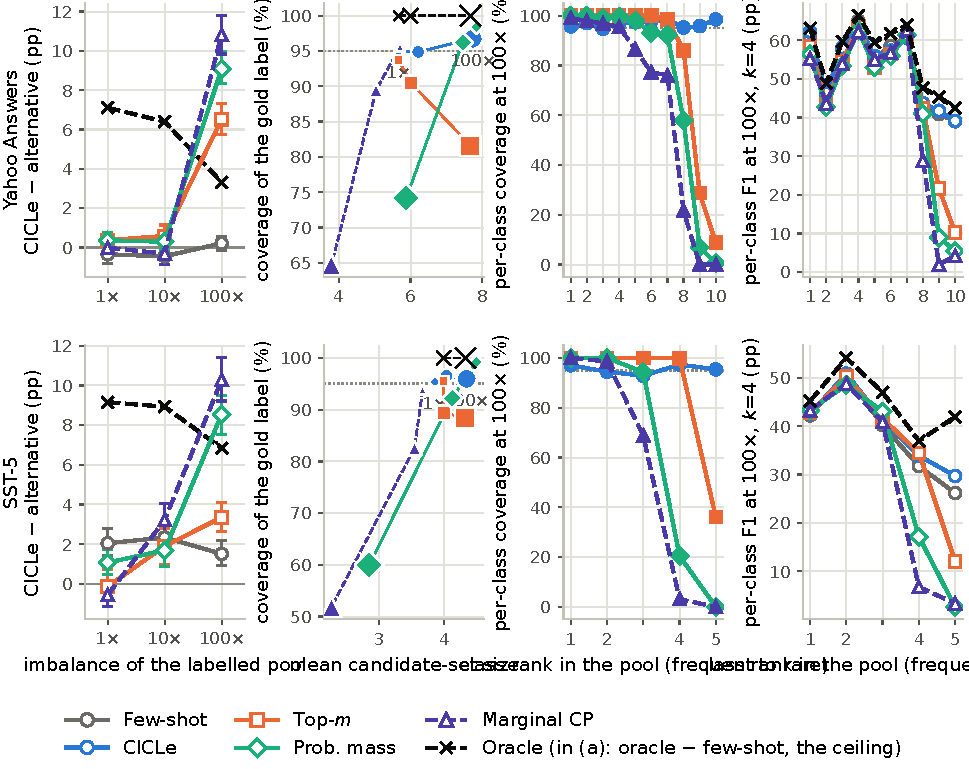
\includegraphics[width=\textwidth]{figures/fig_app_narrowing_fixed.pdf}
  \caption{Figure~\ref{fig:main_narrowing} for the Fixed retrieval variant, with the same aggregation (36 pairs per point on the left, one run per seed on the right).}
  \label{fig:imbalance_fixed}
\end{figure*}


\section{Per-Model Results}
\label{app:models}

Table~\ref{tab:per_model} breaks the main comparison down by model.
The pilot reported, with Fixed retrieval, $-2.07$ for Ministral-3B and $-2.95$ for Qwen2.5-7B on Yahoo Answers, $-1.62$ for Ministral-3B and $-1.20$ for Qwen2.5-3B on SST-5, and positive values for the three other models everywhere. Under the corrected protocol those four cells are $-0.17$ (n.s.), $+0.05$ (n.s.), $+3.36$ and $+0.40$ (n.s.).

% Table D1 (appendix). Body generated by make_figures.py (tabD1).
\begin{table*}[t]
  \centering
  \scriptsize
  \setlength{\tabcolsep}{3pt}
  \resizebox{\textwidth}{!}{% Table D1. CICLe minus few-shot per model, all k pooled (12 pairs, Ohsumed 6), 95% paired bootstrap CI. F = Fixed, PC = Per-Class.
\begin{tabular}{lccccccccc}
\toprule
Model & Yahoo Answers F & Yahoo Answers PC & SST-5 F & SST-5 PC & SemEval-18 F & SemEval-18 PC & GoEmotions F & GoEmotions PC & Ohsumed F \\
\midrule
Llama-3.2-3B & \textbf{-2.33} {\scriptsize [-3.13, -1.53]} & \textbf{+0.82} {\scriptsize [+0.22, +1.42]} & \textbf{+3.85} {\scriptsize [+2.80, +4.92]} & \textbf{+3.17} {\scriptsize [+2.14, +4.24]} & \textbf{+0.50} {\scriptsize [+0.02, +0.96]} & \textbf{+0.92} {\scriptsize [+0.41, +1.43]} & \textbf{+0.92} {\scriptsize [+0.26, +1.62]} & \textbf{+2.46} {\scriptsize [+1.39, +3.47]} & -0.33\,\textsuperscript{n.s.} {\scriptsize [-1.53, +0.98]} \\
Ministral-3B & -0.17\,\textsuperscript{n.s.} {\scriptsize [-1.09, +0.77]} & \textbf{+3.40} {\scriptsize [+2.55, +4.25]} & \textbf{+3.36} {\scriptsize [+2.31, +4.43]} & \textbf{+1.33} {\scriptsize [+0.33, +2.36]} & \textbf{+0.74} {\scriptsize [+0.24, +1.23]} & \textbf{+0.62} {\scriptsize [+0.13, +1.11]} & +0.47\,\textsuperscript{n.s.} {\scriptsize [-0.40, +1.55]} & \textbf{+1.32} {\scriptsize [+0.49, +2.14]} & \textbf{+1.66} {\scriptsize [+0.33, +3.08]} \\
Qwen2.5-3B & \textbf{+1.99} {\scriptsize [+1.23, +2.79]} & \textbf{+2.14} {\scriptsize [+1.35, +2.92]} & +0.40\,\textsuperscript{n.s.} {\scriptsize [-0.60, +1.40]} & \textbf{+1.12} {\scriptsize [+0.03, +2.23]} & +0.12\,\textsuperscript{n.s.} {\scriptsize [-0.28, +0.49]} & +0.16\,\textsuperscript{n.s.} {\scriptsize [-0.31, +0.60]} & +0.39\,\textsuperscript{n.s.} {\scriptsize [-0.26, +1.11]} & \textbf{+0.95} {\scriptsize [+0.19, +1.75]} & \textbf{+4.71} {\scriptsize [+3.20, +6.65]} \\
Mistral-7B & \textbf{-0.69} {\scriptsize [-1.31, -0.06]} & +0.08\,\textsuperscript{n.s.} {\scriptsize [-0.58, +0.75]} & -0.42\,\textsuperscript{n.s.} {\scriptsize [-1.27, +0.47]} & -0.54\,\textsuperscript{n.s.} {\scriptsize [-1.48, +0.42]} & \textbf{+0.85} {\scriptsize [+0.39, +1.31]} & \textbf{+0.73} {\scriptsize [+0.22, +1.23]} & \textbf{+0.73} {\scriptsize [+0.03, +1.40]} & +0.15\,\textsuperscript{n.s.} {\scriptsize [-0.63, +1.10]} & -0.13\,\textsuperscript{n.s.} {\scriptsize [-1.32, +1.12]} \\
Qwen2.5-7B & +0.05\,\textsuperscript{n.s.} {\scriptsize [-0.44, +0.54]} & \textbf{+1.24} {\scriptsize [+0.67, +1.84]} & \textbf{+1.49} {\scriptsize [+0.64, +2.35]} & \textbf{+0.96} {\scriptsize [+0.07, +1.85]} & \textbf{+0.48} {\scriptsize [+0.05, +0.93]} & -0.29\,\textsuperscript{n.s.} {\scriptsize [-0.76, +0.21]} & +0.69\,\textsuperscript{n.s.} {\scriptsize [-0.35, +2.02]} & +0.45\,\textsuperscript{n.s.} {\scriptsize [-0.59, +1.50]} & +0.49\,\textsuperscript{n.s.} {\scriptsize [-0.62, +1.61]} \\
Llama-3.1-8B & +0.03\,\textsuperscript{n.s.} {\scriptsize [-0.49, +0.57]} & \textbf{+0.74} {\scriptsize [+0.20, +1.30]} & \textbf{+1.94} {\scriptsize [+1.06, +2.81]} & +0.35\,\textsuperscript{n.s.} {\scriptsize [-0.59, +1.28]} & +0.45\,\textsuperscript{n.s.} {\scriptsize [-0.01, +0.90]} & \textbf{+0.65} {\scriptsize [+0.14, +1.16]} & +0.32\,\textsuperscript{n.s.} {\scriptsize [-0.52, +1.18]} & +0.20\,\textsuperscript{n.s.} {\scriptsize [-0.76, +1.20]} & +0.51\,\textsuperscript{n.s.} {\scriptsize [-0.65, +1.61]} \\
\bottomrule
\end{tabular}
}
  \caption{CICLe minus few-shot prompting per model, paired over all $k$ and three seeds (12 pairs, Ohsumed 6), with 95\% bootstrap intervals over test instances. F = Fixed, PC = Per-Class. Bold marks intervals that exclude zero.}
  \label{tab:per_model}
\end{table*}


\section{Ablations and the Miscoverage Level}
\label{app:ablations}

Table~\ref{tab:ablation} varies the embedding, the classifier and $\alpha$ with Llama-3.1-8B and Llama-3.2-3B on the four short-text datasets, and Figure~\ref{fig:alpha} plots the $\alpha$ rows.
Few-shot prompting uses the same embedding for retrieval as the CICLe run it is paired with, so the difference isolates the narrowing step.

% Table E1 (appendix). Body generated by make_figures.py (tabE1).
\begin{table*}[t]
  \centering
  \footnotesize
  \setlength{\tabcolsep}{4pt}
  \resizebox{\textwidth}{!}{% Table E1. Llama-3.1-8B and Llama-3.2-3B, both retrieval variants, k in {1,4}, 3 seeds (24 cells). Few-shot uses the same embedding for retrieval. Delta = CICLe - few-shot, paired bootstrap CI.
\begin{tabular}{lllrrrcrrr}
\toprule
Dataset & Embedding & Classifier & $\alpha$ & CICLe & few-shot & $\Delta$ & coverage (\%) & set size & no LLM call (\%) \\
\midrule
Yahoo Answers & contriever & LR & 0.05 & 57.8 & 58.1 & -0.28\,\textsuperscript{n.s.} {\scriptsize [-0.74, +0.20]} & 95.6 & 5.32 & 5.8 \\
 & minilm & LR & 0.05 & 59.4 & 59.8 & -0.37\,\textsuperscript{n.s.} {\scriptsize [-0.82, +0.08]} & 95.0 & 5.67 & 3.4 \\
 & minilm & SVM & 0.05 & 59.8 & 59.8 & -0.05\,\textsuperscript{n.s.} {\scriptsize [-0.50, +0.40]} & 95.6 & 5.79 & 4.7 \\
 & tfidf & LR & 0.05 & 54.5 & 55.2 & \textbf{-0.69} {\scriptsize [-1.10, -0.30]} & 96.1 & 7.97 & 1.1 \\
\addlinespace
 & minilm & LR & 0.01 & 59.8 & 59.8 & -0.07\,\textsuperscript{n.s.} {\scriptsize [-0.30, +0.17]} & 99.1 & 8.98 & 0.0 \\
 & minilm & LR & 0.10 & 60.8 & 59.8 & \textbf{+0.93} {\scriptsize [+0.31, +1.56]} & 90.1 & 4.01 & 9.8 \\
 & minilm & LR & 0.20 & 63.4 & 59.8 & \textbf{+3.57} {\scriptsize [+2.67, +4.48]} & 79.3 & 2.08 & 35.4 \\
\midrule
SST-5 & contriever & LR & 0.05 & 47.0 & 43.3 & \textbf{+3.69} {\scriptsize [+2.82, +4.53]} & 95.5 & 3.34 & 0.5 \\
 & minilm & LR & 0.05 & 45.0 & 42.3 & \textbf{+2.65} {\scriptsize [+1.85, +3.46]} & 95.4 & 3.86 & 0.0 \\
 & minilm & SVM & 0.05 & 44.9 & 42.3 & \textbf{+2.53} {\scriptsize [+1.70, +3.34]} & 96.1 & 3.81 & 0.0 \\
 & tfidf & LR & 0.05 & 42.8 & 41.2 & \textbf{+1.61} {\scriptsize [+0.92, +2.30]} & 95.0 & 4.30 & 0.1 \\
\addlinespace
 & minilm & LR & 0.01 & 43.4 & 42.3 & \textbf{+1.05} {\scriptsize [+0.64, +1.47]} & 99.2 & 4.67 & 0.0 \\
 & minilm & LR & 0.10 & 45.1 & 42.3 & \textbf{+2.75} {\scriptsize [+1.70, +3.76]} & 90.5 & 3.38 & 0.3 \\
 & minilm & LR & 0.20 & 44.9 & 42.3 & \textbf{+2.52} {\scriptsize [+1.24, +3.82]} & 80.3 & 2.71 & 3.0 \\
\midrule
SemEval-18 & contriever & LR & 0.05 & 16.3 & 15.7 & \textbf{+0.56} {\scriptsize [+0.18, +0.95]} & 94.2 & 16.77 & 0.0 \\
 & minilm & LR & 0.05 & 15.8 & 15.3 & \textbf{+0.47} {\scriptsize [+0.13, +0.81]} & 94.4 & 17.12 & 0.0 \\
 & minilm & SVM & 0.05 & 16.0 & 15.3 & \textbf{+0.69} {\scriptsize [+0.34, +1.04]} & 94.9 & 17.13 & 0.0 \\
 & tfidf & LR & 0.05 & 15.1 & 15.0 & +0.11\,\textsuperscript{n.s.} {\scriptsize [-0.15, +0.37]} & 95.1 & 18.06 & 0.0 \\
\addlinespace
 & minilm & LR & 0.01 & 15.4 & 15.3 & +0.12\,\textsuperscript{n.s.} {\scriptsize [-0.07, +0.30]} & 98.8 & 19.42 & 0.0 \\
 & minilm & LR & 0.10 & 16.4 & 15.3 & \textbf{+1.04} {\scriptsize [+0.56, +1.52]} & 88.5 & 14.64 & 0.0 \\
 & minilm & LR & 0.20 & 16.7 & 15.3 & \textbf{+1.36} {\scriptsize [+0.73, +1.96]} & 77.8 & 11.48 & 0.0 \\
\midrule
GoEmotions & contriever & LR & 0.05 & 25.1 & 22.6 & \textbf{+2.46} {\scriptsize [+1.67, +3.19]} & 95.0 & 21.07 & 0.0 \\
 & minilm & LR & 0.05 & 23.3 & 22.4 & \textbf{+0.92} {\scriptsize [+0.31, +1.56]} & 95.4 & 22.10 & 0.0 \\
 & minilm & SVM & 0.05 & 23.7 & 22.4 & \textbf{+1.26} {\scriptsize [+0.64, +2.00]} & 95.1 & 21.75 & 0.0 \\
 & tfidf & LR & 0.05 & 23.1 & 22.5 & \textbf{+0.56} {\scriptsize [+0.04, +1.13]} & 94.5 & 23.74 & 0.0 \\
\addlinespace
 & minilm & LR & 0.01 & 22.9 & 22.4 & \textbf{+0.49} {\scriptsize [+0.14, +0.82]} & 98.8 & 26.74 & 0.0 \\
 & minilm & LR & 0.10 & 23.8 & 22.4 & \textbf{+1.45} {\scriptsize [+0.74, +2.33]} & 90.9 & 18.10 & 0.0 \\
 & minilm & LR & 0.20 & 25.4 & 22.4 & \textbf{+3.02} {\scriptsize [+2.09, +4.24]} & 81.0 & 13.15 & 0.0 \\
\bottomrule
\end{tabular}
}
  \caption{Ablation of the embedding, the classifier and $\alpha$ with Llama-3.1-8B and Llama-3.2-3B, both retrieval variants, $k \in \{1, 4\}$ and three seeds (24 cells). Few-shot prompting retrieves with the same embedding as the CICLe run it is paired with. $\Delta$ = CICLe minus few-shot with its 95\% bootstrap interval. Coverage, set size and the share of instances answered without an LLM call describe the candidate sets.}
  \label{tab:ablation}
\end{table*}

% Figure 3 (column width, two stacked panels): choosing alpha. Spec: figures_and_tables.md. PLACEHOLDER.
% Candidate for the appendix if the page budget bites (presentation_plan.md, resolution (a)).
\begin{figure}[t]
  \centering
  % 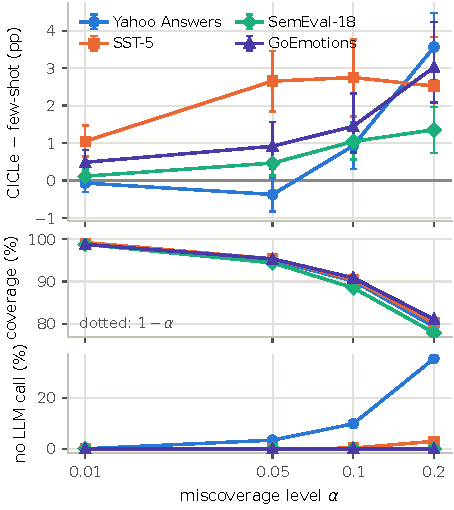
\includegraphics[width=\columnwidth]{figures/alpha.pdf}
  \fbox{\parbox{0.95\columnwidth}{\centering\vspace{3em}\emph{Figure 3 placeholder: $\Delta$ vs.\ few-shot and LLM-skip rate against $\alpha$}\vspace{3em}}}
  \caption{Effect of the miscoverage level $\alpha$. Top: paired difference CICLe minus few-shot, one line per dataset (Llama-3.1-8B and Llama-3.2-3B, 24 cells). Bottom: share of test instances answered by the base classifier alone. Annotations give the empirical coverage at each $\alpha$.}
  \label{fig:alpha}
\end{figure}


\section{Larger Models}
\label{app:large}

Table~\ref{tab:large} runs Mistral-NeMo-12B and Qwen2.5-32B with and without CICLe under the same protocol as the six small models, and lists the best 3B model with CICLe against the 32B model's zero-shot score on the same seed.
% PENDING: 12B and 32B on Ohsumed; Qwen2.5-32B on GoEmotions has one seed.

% Table F1 (appendix). Body generated by make_figures.py (tabF1).
\begin{table*}[t]
  \centering
  \scriptsize
  \setlength{\tabcolsep}{3pt}
  \resizebox{\textwidth}{!}{% Table F1. Mistral-Nemo-12B and Qwen2.5-32B: macro-F1 (mean over the seeds listed), cells 'few-shot / CICLe'; Delta = CICLe - few-shot over k in {1,4}, paired bootstrap CI, (n) cells.
\begin{tabular}{llrcccccc c}
\toprule
Model & Dataset & seeds & Zero-shot & \multicolumn{2}{c}{Fixed} & \multicolumn{2}{c}{Per-Class} & $\Delta$ Fixed & $\Delta$ PC \\
 & & & & $k$=1 & $k$=4 & $k$=1 & $k$=4 & & \\
\midrule
Mistral-Nemo-12B & Yahoo Answers & 42,43,44 & 57.8 & 56.8 / 57.2 & 61.0 / 61.3 & 57.6 / 59.6 & 63.4 / 63.0 & +0.42\,\textsuperscript{n.s.} {\scriptsize [-0.40, +1.24]} (6) & +0.78\,\textsuperscript{n.s.} {\scriptsize [-0.06, +1.62]} (6) \\
Mistral-Nemo-12B & SST-5 & 42,43,44 & 27.5 & 37.6 / 42.5 & 41.6 / 45.1 & 41.7 / 45.6 & 42.0 / 46.9 & \textbf{+4.20} {\scriptsize [+3.08, +5.26]} (6) & \textbf{+4.39} {\scriptsize [+3.14, +5.66]} (6) \\
Mistral-Nemo-12B & SemEval-18 & 42,43,44 & 16.6 & 17.8 / 18.2 & 19.7 / 20.3 & 19.4 / 19.9 & 20.9 / 20.8 & +0.50\,\textsuperscript{n.s.} {\scriptsize [-0.03, +1.02]} (6) & +0.18\,\textsuperscript{n.s.} {\scriptsize [-0.45, +0.83]} (6) \\
Mistral-Nemo-12B & GoEmotions & 42,43,44 & 27.2 & 25.9 / 27.0 & 28.4 / 28.4 & 27.1 / 28.3 & 30.3 / 30.7 & +0.53\,\textsuperscript{n.s.} {\scriptsize [-0.45, +1.48]} (6) & +0.77\,\textsuperscript{n.s.} {\scriptsize [-0.33, +2.05]} (6) \\
\midrule
Qwen2.5-32B & Yahoo Answers & 42,43,44 & 63.2 & 64.0 / 65.0 & 66.4 / 66.9 & 63.9 / 65.2 & 65.8 / 66.4 & \textbf{+0.72} {\scriptsize [+0.15, +1.29]} (6) & \textbf{+0.94} {\scriptsize [+0.29, +1.60]} (6) \\
Qwen2.5-32B & SST-5 & 42,43,44 & 49.3 & 52.1 / 53.8 & 53.5 / 54.8 & 55.5 / 55.9 & 55.2 / 55.5 & \textbf{+1.53} {\scriptsize [+0.49, +2.58]} (6) & +0.32\,\textsuperscript{n.s.} {\scriptsize [-0.68, +1.29]} (6) \\
Qwen2.5-32B & SemEval-18 & 42,43,44 & 15.4 & 17.3 / 17.6 & 19.2 / 19.8 & 19.8 / 20.2 & 20.2 / 20.4 & +0.48\,\textsuperscript{n.s.} {\scriptsize [-0.08, +1.03]} (6) & +0.34\,\textsuperscript{n.s.} {\scriptsize [-0.29, +0.93]} (6) \\
Qwen2.5-32B & GoEmotions & 42,43,44 & 31.5 & 31.2 / 31.4 & 32.7 / 32.4 & 30.7 / 30.5 & 32.4 / 32.2 & -0.05\,\textsuperscript{n.s.} {\scriptsize [-1.01, +0.93]} (6) & -0.20\,\textsuperscript{n.s.} {\scriptsize [-1.01, +0.64]} (6) \\
\midrule
\multicolumn{10}{l}{\emph{Smallest models with CICLe against the largest model without examples (seed 42)}} \\
\multicolumn{10}{l}{Yahoo Answers, best 3B + CICLe PC $k$=4, seed 42: Llama-3.2-3B 61.5, Qwen2.5-32B zero-shot, seed 42: 60.7} \\
\multicolumn{10}{l}{SST-5, best 3B + CICLe PC $k$=4, seed 42: Ministral-3B 51.0, Qwen2.5-32B zero-shot, seed 42: 48.8} \\
\multicolumn{10}{l}{SemEval-18, best 3B + CICLe PC $k$=4, seed 42: Ministral-3B 14.9, Qwen2.5-32B zero-shot, seed 42: 15.3} \\
\multicolumn{10}{l}{GoEmotions, best 3B + CICLe PC $k$=4, seed 42: Qwen2.5-3B 24.4, Qwen2.5-32B zero-shot, seed 42: 32.0} \\
\bottomrule
\end{tabular}
}
  \caption{Mistral-NeMo-12B and Qwen2.5-32B with and without CICLe. Cells give few-shot / CICLe macro-F1, mean over the seeds listed. $\Delta$ = CICLe minus few-shot over $k \in \{1, 4\}$, paired within the model, with 95\% bootstrap intervals and the number of cells. The last rows compare the best 3B model with CICLe (Per-Class, $k = 4$) against the 32B model's zero-shot score on seed 42.}
  \label{tab:large}
\end{table*}


\section{Supervised Baselines and Pool Size}
\label{app:pool}

Table~\ref{tab:baselines} gives the supervised baselines against the LLM pipelines on every dataset and imbalance level, and Figure~\ref{fig:pool} and Table~\ref{tab:pool} give macro-F1 against the size of the labelled pool on the two balanced datasets. % PENDING (rerun): RoBERTa-large rows The base classifier, the retrieval pool and the fine-tuned encoders all see 80\% of the labelled pool, and the calibration split is the remaining 20\% (50 examples at a pool of 250).

% Table 4 (appendix, full width). Body generated by make_figures.py (tab4).
\begin{table*}[t]
  \centering
  \scriptsize
  \setlength{\tabcolsep}{3pt}
  % Table 4. Macro-F1; supervised rows mean over 3 seeds, LLM rows over 6 models x 3 seeds. Zero-shot does not depend on the pool (1x column only). F = Fixed retrieval (Ohsumed has no Per-Class runs). Bold = best per column.
\begin{tabular}{lccccccccc}
\toprule
 & Yahoo Answers 1$\times$ & Yahoo Answers 10$\times$ & Yahoo Answers 100$\times$ & SST-5 1$\times$ & SST-5 10$\times$ & SST-5 100$\times$ & SemEval-18 & GoEmotions & Ohsumed \\
\midrule
MiniLM + LR & \textbf{65.4} & 50.4 & 31.4 & 35.5 & 20.5 & 12.6 & 9.7 & 11.2 & 45.2 \\
RoBERTa-base, fine-tuned & 61.8 & 58.7 & 41.2 & \textbf{51.2} & 44.5 & 31.9 & \textbf{24.5} & \textbf{37.0} & 55.4 \\
RoBERTa-large, fine-tuned & 64.6 & \textbf{61.6} & 44.9 & 39.9 & 35.8 & 32.2 & 23.0 & 27.3 & \textbf{66.1} \\
Zero-shot & 55.3 & -- & -- & 40.3 & -- & -- & 12.2 & 24.9 & 35.9 \\
Few-shot PC, $k$=4 & 61.6 & 59.4 & 54.6 & 46.6 & 44.6 & 40.8 & 15.4 & 24.8 & 50.4\textsuperscript{F} \\
CICLe PC, $k$=4 & 62.7 & 60.3 & 55.4 & 47.5 & \textbf{46.5} & 41.9 & 15.7 & 26.0 & 51.7\textsuperscript{F} \\
Best LLM pipeline & 63.8 {\scriptsize CICLe PC $k$=8} & 60.3 {\scriptsize CICLe PC $k$=4} & \textbf{56.0} {\scriptsize CICLe PC $k$=1} & 47.6 {\scriptsize CICLe PC $k$=2} & \textbf{46.5} {\scriptsize CICLe PC $k$=4} & \textbf{43.4} {\scriptsize CICLe PC $k$=1} & 16.1 {\scriptsize CICLe F $k$=8} & 27.3 {\scriptsize CICLe F $k$=8} & 53.1 {\scriptsize CICLe F $k$=8} \\
\bottomrule
\end{tabular}

  \caption{Supervised baselines against LLM pipelines, macro-F1. Supervised rows are means over three seeds, LLM rows over six models and three seeds. The fixed configuration is Per-Class retrieval at $k = 4$ (Ohsumed: Fixed, marked F). The best pipeline is the best (method, variant, $k$) mean per column and is selected on the test set. Zero-shot prompting does not depend on the pool. The test sample is identical at every imbalance level. Bold marks the best value per column.}
  \label{tab:baselines}
\end{table*}

% Figure P (column width). Generated by make_figures.py (figP).
\begin{figure}[t]
  \centering
  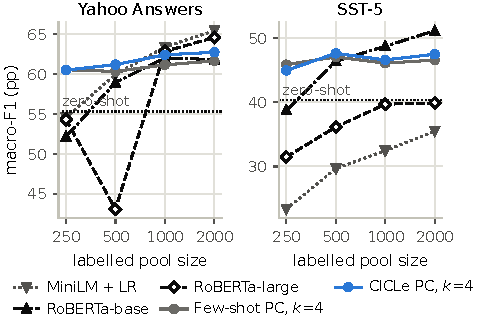
\includegraphics[width=\columnwidth]{figures/pool_size.pdf}
  \caption{Macro-F1 against the size of the labelled pool (log scale) on Yahoo Answers and SST-5. Supervised models are means over three seeds, LLM pipelines (Per-Class, $k = 4$, and the best configuration) over six models and three seeds. Zero-shot prompting, which does not depend on the pool, is the dotted reference line. The test sample is the same at every pool size.}
  \label{fig:pool}
\end{figure}

% Table P (appendix). Body generated by make_figures.py (tabP).
\begin{table*}[t]
  \centering
  \small
  \resizebox{\textwidth}{!}{% Table P. Macro-F1 against the size of the labelled pool (train + calibration; the base classifier, retrieval pool and fine-tuned models all see 80% of it). Supervised rows mean over 3 seeds, LLM rows over 6 models x 3 seeds; the test sample is the same at every pool size. Best pipeline: argmax over (method, variant, k) of the 18-run mean (k in {1,4} below 2,000). Bold = best per row.
\begin{tabular}{lrcccccc}
\toprule
Dataset & labelled pool & MiniLM + LR & RoBERTa-base & RoBERTa-large & Few-shot PC, $k$=4 & CICLe PC, $k$=4 & best LLM pipeline \\
\midrule
Yahoo Answers & 250 & 54.6 & 52.2 & 54.3 & \textbf{60.6} & 60.5 & \textbf{60.6} {\scriptsize FS PC $k$=4} \\
 & 500 & 60.0 & 59.0 & 43.1 & 60.3 & \textbf{61.2} & \textbf{61.2} {\scriptsize CICLe PC $k$=4} \\
 & 1,000 & \textbf{63.4} & 62.0 & 62.9 & 61.2 & 62.4 & 62.4 {\scriptsize CICLe PC $k$=4} \\
 & 2,000 & \textbf{65.4} & 61.8 & 64.6 & 61.6 & 62.7 & 63.8 {\scriptsize CICLe PC $k$=8} \\
\midrule
SST-5 & 250 & 23.3 & 38.8 & 31.5 & \textbf{45.9} & 45.0 & \textbf{45.9} {\scriptsize FS PC $k$=4} \\
 & 500 & 29.7 & 46.4 & 36.2 & 47.1 & \textbf{47.6} & \textbf{47.6} {\scriptsize CICLe PC $k$=4} \\
 & 1,000 & 32.5 & \textbf{48.8} & 39.7 & 46.1 & 46.6 & 46.6 {\scriptsize CICLe PC $k$=4} \\
 & 2,000 & 35.5 & \textbf{51.2} & 39.9 & 46.6 & 47.5 & 47.6 {\scriptsize CICLe PC $k$=2} \\
\bottomrule
\end{tabular}
}
  \caption{Macro-F1 against the size of the labelled pool (training plus calibration, split 80/20). Supervised rows are means over three seeds, LLM rows over six models and three seeds, and the test sample is the same at every pool size. The best pipeline is selected on the test set among $k \in \{1, 4\}$ below 2,000 labels. Bold marks the best value per row. The RoBERTa-large rows are being rerun with a lower learning rate.}
  \label{tab:pool}
\end{table*}


\section{Per-Instance Analyses}
\label{app:instances}

Table~\ref{tab:fixes} pairs every test instance between CICLe and few-shot prompting at $k = 4$ and splits the fixes and breaks by whether the gold label was in the candidate set and by whether the few-shot answer was.
Table~\ref{tab:invalid} gives the invalid-output rate per model and dataset for every method, Table~\ref{tab:invalid_raw} the most frequent unparseable outputs (emoji replaced by ``[emoji]'' for typesetting), and Table~\ref{tab:examples} qualitative examples of instances that narrowing fixed or broke.
The most frequent unparseable outputs are labels of the wrong granularity (``Relationships'' for Family, ``Neurological Diseases'' for a 23-way Ohsumed category), emoji outside the label set and refusals, which supports the reading of Section~\ref{sec:res-protocol} that the pilot's failures were failures of the prompt rather than of the method.

% Table G1 (appendix). Body generated by make_figures.py (tabG1).
\begin{table*}[t]
  \centering
  \scriptsize
  \setlength{\tabcolsep}{3pt}
  \resizebox{\textwidth}{!}{% Table G1. CICLe k=4 vs few-shot k=4, same retrieval variant, 6 models x 3 seeds x 1,000 instances. fixed = CICLe right & few-shot wrong; broken = the reverse. 'gold outside set' / 'few-shot answer outside set': share of pairs, then fixed and broken as % of that subset.
\begin{tabular}{llrrrrrrrrrrr}
\toprule
Variant & Retr. & pairs & fixed & broken & both right & both wrong & \multicolumn{3}{c}{gold outside set} & \multicolumn{3}{c}{few-shot answer outside set} \\
 & & & \multicolumn{4}{c}{(\% of pairs)} & share & fixed & broken & share & fixed & broken \\
\midrule
Yahoo Answers & Per-Class & 18,000 & 4.7 & 3.4 & 58.0 & 33.8 & 5.0 & 0.0 & 4.1 & 5.0 & 39.5 & 4.1 \\
Yahoo Answers & Fixed & 18,000 & 4.2 & 4.3 & 53.7 & 37.8 & 5.0 & 0.0 & 5.6 & 7.8 & 31.1 & 3.5 \\
SST-5 & Per-Class & 18,000 & 6.9 & 6.1 & 42.2 & 44.7 & 4.6 & 0.6 & 35.6 & 6.3 & 34.9 & 26.1 \\
SST-5 & Fixed & 18,000 & 7.0 & 5.8 & 40.4 & 46.8 & 4.6 & 0.8 & 33.2 & 6.2 & 35.0 & 24.9 \\
SemEval-18 & Per-Class & 18,000 & 3.1 & 3.2 & 18.8 & 74.9 & 5.6 & 0.0 & 11.1 & 7.6 & 10.1 & 8.2 \\
SemEval-18 & Fixed & 18,000 & 2.7 & 2.6 & 18.5 & 76.2 & 5.6 & 0.0 & 8.8 & 10.3 & 7.0 & 4.8 \\
GoEmotions & Per-Class & 18,000 & 4.6 & 3.2 & 22.6 & 69.6 & 4.6 & 0.0 & 8.3 & 8.7 & 15.2 & 4.4 \\
GoEmotions & Fixed & 18,000 & 4.1 & 3.0 & 24.1 & 68.8 & 4.6 & 0.0 & 7.6 & 10.3 & 14.0 & 3.4 \\
Ohsumed & Fixed & 18,000 & 7.2 & 4.9 & 52.2 & 35.7 & 3.6 & 0.0 & 15.4 & 12.9 & 33.5 & 4.3 \\
Yahoo Answers 100$\times$ & Per-Class & 18,000 & 3.7 & 2.6 & 52.3 & 41.4 & 3.3 & 0.0 & 9.9 & 5.5 & 27.7 & 5.8 \\
Yahoo Answers 100$\times$ & Fixed & 18,000 & 3.5 & 3.0 & 49.6 & 44.0 & 3.3 & 0.0 & 9.5 & 7.0 & 23.1 & 4.5 \\
SST-5 100$\times$ & Per-Class & 18,000 & 4.7 & 4.1 & 39.7 & 51.6 & 4.0 & 0.0 & 40.8 & 5.1 & 34.4 & 32.2 \\
SST-5 100$\times$ & Fixed & 18,000 & 5.1 & 4.5 & 37.2 & 53.2 & 4.0 & 0.7 & 40.4 & 5.8 & 35.0 & 27.9 \\
Yahoo Answers (renamed) & Per-Class & 18,000 & 9.2 & 5.6 & 43.4 & 41.8 & 5.2 & 0.0 & 7.6 & 11.7 & 41.1 & 3.4 \\
Yahoo Answers (renamed) & Fixed & 18,000 & 8.8 & 5.2 & 36.0 & 50.0 & 5.2 & 0.0 & 7.0 & 18.4 & 30.5 & 2.0 \\
SST-5 (renamed) & Per-Class & 18,000 & 7.6 & 6.1 & 32.2 & 54.1 & 4.6 & 0.0 & 33.0 & 8.1 & 34.8 & 18.8 \\
SST-5 (renamed) & Fixed & 18,000 & 7.6 & 4.6 & 28.8 & 59.0 & 4.6 & 0.0 & 18.8 & 9.8 & 32.3 & 8.8 \\
SemEval-18 (renamed) & Per-Class & 18,000 & 3.7 & 2.9 & 10.7 & 82.7 & 5.6 & 0.0 & 7.6 & 6.2 & 13.3 & 6.8 \\
SemEval-18 (renamed) & Fixed & 18,000 & 2.8 & 2.0 & 9.3 & 85.9 & 5.6 & 0.0 & 5.9 & 13.4 & 7.7 & 2.4 \\
GoEmotions (renamed) & Per-Class & 18,000 & 5.4 & 3.7 & 14.4 & 76.5 & 4.5 & 0.0 & 6.5 & 14.7 & 13.0 & 2.0 \\
GoEmotions (renamed) & Fixed & 18,000 & 4.2 & 3.6 & 13.1 & 79.1 & 4.5 & 0.0 & 5.0 & 14.2 & 11.7 & 1.6 \\
Ohsumed (renamed) & Fixed & 18,000 & 8.7 & 6.3 & 40.7 & 44.3 & 3.7 & 0.0 & 11.6 & 20.6 & 29.7 & 2.1 \\
\bottomrule
\end{tabular}
}
  \caption{Fixes and breaks. CICLe at $k = 4$ against few-shot prompting at $k = 4$ with the same retrieval variant, six models, three seeds and 1,000 instances (18,000 pairs). Fixed = CICLe right and few-shot wrong, broken = the reverse. The right-hand blocks give the share of pairs whose gold label, or whose few-shot answer, lies outside the candidate set, and the fixed and broken rates within that subset.}
  \label{tab:fixes}
\end{table*}

% Table G2 (appendix). Body generated by make_figures.py (tabG2).
\begin{table*}[t]
  \centering
  \scriptsize
  \setlength{\tabcolsep}{3pt}
  \resizebox{\textwidth}{!}{% Table G2. Invalid (unparseable) outputs per model and dataset, reference setting; mean and maximum over (variant, k, seed) runs of each method.
\begin{tabular}{lccccc}
\toprule
Model & Yahoo Answers & SST-5 & SemEval-18 & GoEmotions & Ohsumed \\
 & \multicolumn{5}{c}{mean (max) invalid rate in \%: zero-shot / few-shot / CICLe} \\
\midrule
Llama-3.2-3B & 1.7 (1.9) / 0.2 (0.7) / 0.3 (1.3) & 0.0 (0.0) / 0.0 (0.1) / 0.0 (0.1) & 0.4 (0.5) / 1.5 (5.1) / 1.5 (6.1) & 0.2 (0.2) / 0.6 (1.3) / 0.4 (0.8) & 2.5 (2.7) / 0.6 (1.3) / 0.1 (0.7) \\
Ministral-3B & 1.6 (2.0) / 0.3 (2.0) / 0.2 (0.6) & 0.0 (0.0) / 0.0 (0.0) / 0.0 (0.0) & 0.1 (0.2) / 0.6 (1.3) / 0.4 (0.9) & 0.1 (0.1) / 0.2 (0.5) / 0.1 (0.3) & 0.6 (0.7) / 0.8 (1.4) / 0.3 (0.6) \\
Qwen2.5-3B & 11.7 (13.2) / 9.9 (15.7) / 4.7 (10.2) & 0.0 (0.0) / 0.0 (0.1) / 0.0 (0.1) & 9.1 (9.9) / 14.6 (24.5) / 13.5 (22.4) & 4.1 (4.9) / 3.9 (6.7) / 3.4 (5.9) & 22.2 (23.7) / 20.7 (30.3) / 6.6 (8.9) \\
Mistral-7B & 10.4 (10.8) / 2.7 (7.9) / 1.9 (7.1) & 0.1 (0.1) / 0.0 (0.1) / 0.1 (0.8) & 7.4 (7.9) / 5.2 (8.9) / 4.6 (7.8) & 7.5 (8.0) / 5.2 (10.5) / 3.7 (6.9) & 2.9 (3.4) / 3.1 (5.9) / 0.5 (0.9) \\
Qwen2.5-7B & 11.1 (11.4) / 2.6 (5.0) / 1.7 (6.8) & 0.0 (0.0) / 0.0 (0.2) / 0.0 (0.2) & 12.3 (13.4) / 6.4 (9.9) / 6.6 (12.5) & 5.5 (6.3) / 6.2 (7.8) / 5.0 (6.7) & 2.5 (2.8) / 3.2 (6.5) / 0.9 (1.5) \\
Llama-3.1-8B & 0.4 (0.5) / 0.1 (0.3) / 0.0 (0.1) & 0.0 (0.0) / 0.0 (0.0) / 0.0 (0.0) & 1.1 (1.4) / 0.8 (1.3) / 0.7 (1.2) & 0.9 (1.0) / 0.8 (1.4) / 0.6 (1.1) & 0.7 (1.0) / 0.2 (0.6) / 0.0 (0.1) \\
Mistral-Nemo-12B & 4.1 (4.4) / 0.7 (2.2) / 0.2 (0.8) & 0.0 (0.0) / 0.0 (0.0) / 0.0 (0.1) & 5.6 (5.8) / 2.3 (5.5) / 2.4 (5.4) & 1.0 (1.2) / 1.0 (2.2) / 0.8 (1.3) & -- / -- / -- \\
Qwen2.5-32B & 3.2 (3.7) / 0.5 (1.1) / 0.4 (1.1) & 0.0 (0.0) / 0.0 (0.0) / 0.0 (0.0) & 13.0 (14.2) / 6.0 (9.0) / 5.2 (7.9) & 2.8 (3.1) / 2.7 (4.0) / 1.8 (2.7) & -- / -- / -- \\
\bottomrule
\end{tabular}
}
  \caption{Invalid (unparseable) outputs per model and dataset at the reference setting, mean and maximum over the (variant, $k$, seed) runs of each method.}
  \label{tab:invalid}
\end{table*}

% Table G2b (appendix). Body generated by make_figures.py (tabG2); emoji replaced by [emoji] for pdfLaTeX.
\begin{table*}[t]
  \centering
  \small
  % Table G2b. Raw outputs that matched no label (first 60 characters), pooled over the five main datasets, all methods, reference setting.
\begin{tabular}{lrp{0.75\linewidth}}
\toprule
Model & invalid outputs & most frequent raw outputs (count) \\
\midrule
Llama-3.2-3B & 1,392 & \texttt{discomfort} (90), \texttt{[emoji]} (81), \texttt{Neurological Diseases} (77), \texttt{[emoji]} (69), \texttt{I cannot predict the class for} (40), \texttt{[emoji]} (39), \texttt{[emoji]} (35), \texttt{[emoji]} (30) \\
Ministral-3B & 704 & \texttt{Religion} (52), \texttt{[emoji] *(Note: While not in your provided} (41), \texttt{Mycoses} (40), \texttt{**Mycoses**} (18), \texttt{[emoji] *(Note: The provided emoji list} (11), \texttt{[emoji]} (10), \texttt{[emoji] *(Note: The provided emoji list} (9), \texttt{nostalgia *(not listed in your} (9) \\
Qwen2.5-3B & 18,367 & \texttt{[emoji]} (1,338), \texttt{Neurological Diseases} (1,328), \texttt{[emoji]} (1,023), \texttt{Relationships} (666), \texttt{[emoji]} (648), \texttt{[emoji]} (617), \texttt{[emoji]} (565), \texttt{[emoji]} (528) \\
Mistral-7B & 7,322 & \texttt{Based on the provided text} (106), \texttt{It is difficult to accurately} (84), \texttt{appreciation} (84), \texttt{concern} (81), \texttt{[emoji]} (77), \texttt{discrimination} (69), \texttt{[emoji] (This emoji represents a party} (61), \texttt{anxiety} (60) \\
Qwen2.5-7B & 8,853 & \texttt{[emoji]} (758), \texttt{disbelief} (418), \texttt{advice} (311), \texttt{discomfort} (265), \texttt{Neurological Diseases} (235), \texttt{[emoji]} (220), \texttt{Religion} (213), \texttt{[emoji]} (168) \\
Llama-3.1-8B & 870 & \texttt{anxiety} (87), \texttt{discomfort} (65), \texttt{[emoji]} (64), \texttt{concern} (40), \texttt{nostalgia} (30), \texttt{Neurological Diseases} (25), \texttt{[emoji]} (21), \texttt{nostalgia is not in the list} (19) \\
Mistral-Nemo-12B & 1,207 & \texttt{[emoji]} (94), \texttt{gratuity} (54), \texttt{History} (46), \texttt{Religion} (46), \texttt{[emoji]} (42), \texttt{disbelief} (37), \texttt{[emoji]} (36), \texttt{[emoji]} (36) \\
Qwen2.5-32B & 2,561 & \texttt{[emoji]} (319), \texttt{[emoji]} (103), \texttt{disbelief} (88), \texttt{[emoji]} (85), \texttt{[emoji]} (79), \texttt{nostalgia It seems that the} (65), \texttt{disbelief However, since "dis} (37), \texttt{[emoji]} (35) \\
\bottomrule
\end{tabular}

  \caption{The most frequent raw outputs that matched no label (first 60 characters), pooled over the five main datasets and all methods at the reference setting. Emoji are shown as [emoji].}
  \label{tab:invalid_raw}
\end{table*}

% Table G3 (appendix). Body generated by make_figures.py (tabG3).
\begin{table*}[t]
  \centering
  \scriptsize
  \setlength{\tabcolsep}{2pt}
  % Table G3. Yahoo Answers and GoEmotions, Llama-3.1-8B, seed 42, Per-Class k=4; three instances per case sampled with a fixed seed.
\begin{tabular}{p{0.14\linewidth}p{0.36\linewidth}p{0.08\linewidth}p{0.2\linewidth}p{0.08\linewidth}p{0.08\linewidth}}
\toprule
Case & Text & Gold & Candidate set & Few-shot & CICLe \\
\midrule
fixed: few-shot answered outside the set & My favourite one is the wings on his back. I know his got 9 altogether, but what are they? & Sports & Education, Entertainment, Sports & Culture & Sports \\
fixed: few-shot answered outside the set & I have a relatively new Dell and it has some spots on it. I don't know what's safe to use.... & Tech & Tech & Health & (no LLM call) \\
fixed: few-shot answered outside the set & nothing seems to work! & Tech & Business, Culture, Education, Entertainment, Health, Science, Tech & Family & Tech \\
broken: gold outside the set & I just started celebrationg holidays my son is turning one soon. I have never attended a childs birthday party. Does anyone have ideas? He (... & Family & Culture, Education, Entertainment, Health, Science, Sports, Tech & Family & Education \\
broken: gold outside the set & I Help with my home work ?Why do we argue about gay marriage? why people argue this? and give 3 reasons why we argue and explain?and conclus... & Family & Business, Culture, Education, Entertainment, Politics, Science, Sports, Tech & Family & Education \\
broken: gold outside the set & Can we ever compensate for the love and care they gave us in our childhood and how many sacrifices they did towards our upbringing? & Family & Culture, Education, Politics & Family & Culture \\
broken: switched inside the set & Hi ladies, Just curious when and HOW did you know if you were a lesbian; were you ashamed?? & Family & Business, Culture, Education, Entertainment, Family, Health, Tech & Family & Culture \\
broken: switched inside the set & Who can tell the names of atleast seven characters? if you can you win...nothing you just get points for answering & Entertainment & Culture, Education, Entertainment, Science, Sports, Tech & Entertainment & Education \\
broken: switched inside the set & I watched it last night and it was the first episode...I hope and pray that the black woman who is preaching the "Words of God"...remind you... & Culture & Culture, Entertainment & Culture & Entertainment \\
\midrule
fixed: few-shot answered outside the set & Help, help, I'm being repressed! & fear & annoyance, caring, confusion, desire, disappointment, disgust, embarrassment, fear, grief, nervousness, neutral, optimism, pride, realization, relief, remorse, sadness & anger & fear \\
fixed: few-shot answered outside the set & Lawson's Sip of Sunshine! Excellent Vermont beer. & admiration & admiration, amusement, caring, curiosity, desire, disappointment, disgust, embarrassment, excitement, fear, gratitude, grief, joy, love, nervousness, neutral, optimism, pride, realization, relief, remorse, sadness, surprise & approval & admiration \\
fixed: few-shot answered outside the set & Stuck on icy stairs. & neutral & admiration, annoyance, caring, confusion, curiosity, desire, disappointment, disgust, embarrassment, excitement, fear, grief, joy, nervousness, neutral, optimism, pride, realization, relief, remorse, surprise & disapproval & neutral \\
broken: gold outside the set & Please treat me with modern medicine. I have gastroparisis. & caring & admiration, annoyance, approval, curiosity, disappointment, disapproval, disgust, excitement, fear, grief, joy, love, nervousness, neutral, optimism, pride, realization, relief, remorse, sadness, surprise & caring & approval \\
broken: gold outside the set & Wasnt much to ruin. & neutral & admiration, amusement, anger, annoyance, approval, caring, confusion, curiosity, desire, disappointment, disapproval, disgust, embarrassment, excitement, fear, gratitude, grief, joy, nervousness, optimism, pride, realization, relief, remorse, surprise & neutral & amusement \\
broken: gold outside the set & Someone with erectile dysfunction already can't (conventionally) orgasm. What the fuck are you talking about? & anger & admiration, amusement, annoyance, approval, confusion, curiosity, desire, disappointment, disapproval, disgust, embarrassment, fear, grief, joy, love, nervousness, neutral, optimism, pride, realization, relief, remorse, sadness, surprise & anger & disapproval \\
broken: switched inside the set & Hope gallery for sure, had [NAME] do mine and a good friend back in 2015. Not sure if he's still there, however. & optimism & admiration, amusement, approval, caring, confusion, curiosity, desire, disappointment, disgust, embarrassment, excitement, fear, gratitude, grief, joy, love, nervousness, optimism, realization, relief, remorse, surprise & optimism & curiosity \\
broken: switched inside the set & Tu eres very nice man & admiration & admiration, amusement, anger, annoyance, approval, confusion, disappointment, disgust, embarrassment, excitement, fear, gratitude, grief, joy, love, nervousness, optimism, pride, realization, relief, remorse, sadness, surprise & admiration & gratitude \\
broken: switched inside the set & I've exposed on social media. It made me feel better so I don't care what anyway has to say about it. & relief & admiration, amusement, anger, annoyance, approval, caring, curiosity, disappointment, disapproval, disgust, embarrassment, excitement, fear, gratitude, grief, nervousness, neutral, optimism, pride, realization, relief, remorse, sadness, surprise & relief & optimism \\
\bottomrule
\end{tabular}

  \caption{Qualitative examples from Yahoo Answers and GoEmotions, Llama-3.1-8B, seed 42, Per-Class $k = 4$. Three instances per case, sampled with a fixed seed, texts truncated to 140 characters.}
  \label{tab:examples}
\end{table*}


\section{Dataset Details}
\label{app:data}

Table~\ref{tab:imbalance_counts} lists the class order and training-pool counts under controlled imbalance for every seed. Class sizes follow a geometric schedule between the largest and the smallest class, with at least five examples per class before the 80/20 split, and the class order is a random permutation drawn from the seed, so the rare classes differ between seeds and the per-class results of Figure~\ref{fig:imbalance} are aggregated by frequency rank.
Table~\ref{tab:relabel_words} gives the nonsense-word mapping used for label renaming. The words are six-letter consonant-vowel strings generated with a fixed seed, no two sharing a four-letter prefix, so that the prefix matching of the parser cannot confuse them.

% Table H1 (appendix). Body generated by make_figures.py (tabH1).
\begin{table*}[t]
  \centering
  \small
  % Table H1. Class order and training-pool counts (after the 80/20 calibration split) under controlled imbalance; the class order is a seed-dependent permutation.
\begin{tabular}{llrp{0.7\linewidth}}
\toprule
Dataset & Imbalance & Seed & class: training count (descending) \\
\midrule
Yahoo Answers & 10$\times$ & 42 & Sports 391, Business 303, Culture 234, Entertainment 182, Education 141, Health 109, Tech 84, Politics 66, Science 50, Family 39 \\
Yahoo Answers & 10$\times$ & 43 & Health 391, Family 303, Politics 234, Sports 182, Entertainment 141, Science 109, Tech 84, Business 66, Culture 50, Education 39 \\
Yahoo Answers & 10$\times$ & 44 & Education 391, Culture 303, Health 234, Sports 182, Tech 141, Science 109, Family 84, Business 66, Politics 50, Entertainment 39 \\
Yahoo Answers & 100$\times$ & 42 & Sports 645, Business 386, Culture 232, Entertainment 139, Education 83, Health 50, Tech 30, Politics 18, Science 10, Family 6 \\
Yahoo Answers & 100$\times$ & 43 & Health 645, Family 386, Politics 232, Sports 139, Entertainment 83, Science 50, Tech 30, Business 18, Culture 10, Education 6 \\
Yahoo Answers & 100$\times$ & 44 & Education 645, Culture 386, Health 232, Sports 139, Tech 83, Science 50, Family 30, Business 18, Politics 10, Entertainment 6 \\
SST-5 & 10$\times$ & 42 & very positive 742, neutral 418, positive 234, negative 132, very negative 74 \\
SST-5 & 10$\times$ & 43 & very positive 742, negative 418, neutral 234, very negative 132, positive 74 \\
SST-5 & 10$\times$ & 44 & neutral 742, positive 418, very negative 234, very positive 132, negative 74 \\
SST-5 & 100$\times$ & 42 & positive 1098, very negative 347, negative 110, neutral 34, very positive 11 \\
SST-5 & 100$\times$ & 43 & neutral 1098, positive 347, very negative 110, negative 34, very positive 11 \\
SST-5 & 100$\times$ & 44 & neutral 1098, positive 347, very negative 110, very positive 34, negative 11 \\
\bottomrule
\end{tabular}

  \caption{Class order and training-pool counts (after the 80/20 calibration split) under controlled imbalance for every seed. The class order is a permutation drawn from the seed.}
  \label{tab:imbalance_counts}
\end{table*}

% Table H1b (appendix). Body generated by make_figures.py (tabH1).
\begin{table*}[t]
  \centering
  \small
  % Table H1b. Nonsense-word mapping used for label renaming (same for all seeds).
\begin{tabular}{lp{0.8\linewidth}}
\toprule
Dataset & original name $\to$ nonsense word \\
\midrule
Yahoo Answers & Business $\to$ zovobi, Culture $\to$ pomini, Education $\to$ repeke, Entertainment $\to$ varipu, Family $\to$ fidazi, Health $\to$ nudimi, Politics $\to$ reponu, Science $\to$ kavuba, Sports $\to$ totaro, Tech $\to$ zigita \\
GoEmotions & admiration $\to$ zovobi, amusement $\to$ pomini, anger $\to$ repeke, annoyance $\to$ varipu, approval $\to$ fidazi, caring $\to$ nudimi, confusion $\to$ reponu, curiosity $\to$ kavuba, desire $\to$ totaro, disappointment $\to$ zigita, disapproval $\to$ gugeve, disgust $\to$ vunadi, embarrassment $\to$ podipi, excitement $\to$ tapizu, fear $\to$ gupuko, gratitude $\to$ duvolu, grief $\to$ gifeze, joy $\to$ busina, love $\to$ defaza, nervousness $\to$ tusozu, neutral $\to$ kuveze, optimism $\to$ suzori, pride $\to$ nosidi, realization $\to$ ranusi, relief $\to$ zegati, remorse $\to$ delelo, sadness $\to$ zadeze, surprise $\to$ busura \\
\bottomrule
\end{tabular}

  \caption{Nonsense-word mapping used for label renaming, the same for all seeds. SST-5, SemEval-18 and Ohsumed use the same word list in alphabetical order of the original names.}
  \label{tab:relabel_words}
\end{table*}


\section{Full Result Grids}
\label{app:full}

Tables~\ref{tab:grid_yahoo} to~\ref{tab:grid_ohsumed_relabel} give every method, retrieval variant and $k$ for each dataset variant at the reference setting, with accuracy, invalid-output rate, mean number of examples and mean prompt tokens per LLM call, as means over the runs of the six small models.

% Table B (appendix), yahoo-answers. Body generated by make_figures.py (tabB).
\begin{table*}[t]
  \centering
  \footnotesize
  % Table B: yahoo-answers, six small models, reference setting (MiniLM, LR, alpha 0.05); means over runs. A row with fewer than 18 runs (3 for the supervised rows) is an incomplete, still-running configuration.
\begin{tabular}{llrrrrrrr}
\toprule
Method & Retrieval & $k$ & runs & macro-F1 & acc. & invalid (\%) & shots & tokens \\
\midrule
MiniLM + LR & -- & -- & 3 & 65.4 & 66.0 & 0.0 & 0.0 & 0 \\
RoBERTa-base (fine-tuned) & -- & -- & 6 & 63.2 & 63.6 & 0.0 & 0.0 & 0 \\
\midrule
Zero-shot & -- & -- & 18 & 55.3 & 54.6 & 6.1 & 0.0 & 221 \\
\midrule
Few-shot & Fixed & 1 & 18 & 54.8 & 54.0 & 4.8 & 1.0 & 285 \\
Few-shot & Fixed & 2 & 18 & 56.4 & 55.8 & 3.8 & 2.0 & 343 \\
Few-shot & Fixed & 4 & 18 & 58.4 & 58.0 & 2.8 & 4.0 & 455 \\
Few-shot & Fixed & 8 & 18 & 59.8 & 59.7 & 1.7 & 8.0 & 674 \\
Few-shot & Per-Class & 1 & 18 & 57.9 & 57.5 & 2.9 & 10.0 & 700 \\
Few-shot & Per-Class & 2 & 18 & 59.5 & 59.3 & 2.0 & 20.0 & 1,183 \\
Few-shot & Per-Class & 4 & 18 & 61.6 & 61.5 & 1.6 & 40.0 & 2,166 \\
Few-shot & Per-Class & 8 & 18 & 62.2 & 62.1 & 1.5 & 80.0 & 4,168 \\
CICLe & Fixed & 0 & 18 & 56.3 & 55.8 & 3.3 & 0.0 & 212 \\
CICLe & Fixed & 1 & 18 & 54.2 & 53.7 & 2.7 & 1.0 & 276 \\
CICLe & Fixed & 2 & 18 & 56.5 & 56.0 & 2.1 & 2.0 & 334 \\
CICLe & Fixed & 4 & 18 & 58.2 & 57.9 & 1.2 & 4.0 & 447 \\
CICLe & Fixed & 8 & 18 & 59.7 & 59.6 & 0.7 & 8.0 & 666 \\
CICLe & Per-Class & 1 & 18 & 59.5 & 59.2 & 1.3 & 5.8 & 503 \\
CICLe & Per-Class & 2 & 18 & 60.9 & 60.8 & 0.8 & 11.7 & 792 \\
CICLe & Per-Class & 4 & 18 & 62.7 & 62.7 & 0.6 & 23.3 & 1,378 \\
CICLe & Per-Class & 8 & 18 & 63.8 & 63.7 & 0.6 & 46.7 & 2,566 \\
\midrule
Top-$m$ & Fixed & 1 & 18 & 53.9 & 53.5 & 2.5 & 1.0 & 277 \\
Top-$m$ & Fixed & 4 & 18 & 57.8 & 57.5 & 1.0 & 4.0 & 448 \\
Top-$m$ & Per-Class & 1 & 18 & 58.5 & 58.2 & 1.3 & 5.7 & 505 \\
Top-$m$ & Per-Class & 4 & 18 & 62.2 & 62.1 & 0.5 & 22.7 & 1,381 \\
Prob. mass & Fixed & 1 & 18 & 54.0 & 53.4 & 3.7 & 1.0 & 281 \\
Prob. mass & Fixed & 4 & 18 & 57.7 & 57.4 & 2.1 & 4.0 & 452 \\
Prob. mass & Per-Class & 1 & 18 & 58.0 & 57.7 & 2.1 & 7.8 & 604 \\
Prob. mass & Per-Class & 4 & 18 & 61.5 & 61.5 & 1.0 & 31.4 & 1,777 \\
Marginal CP & Fixed & 1 & 18 & 54.4 & 54.0 & 2.5 & 1.0 & 275 \\
Marginal CP & Fixed & 4 & 18 & 58.1 & 57.8 & 1.2 & 4.0 & 445 \\
Marginal CP & Per-Class & 1 & 18 & 59.1 & 59.0 & 1.2 & 6.0 & 509 \\
Marginal CP & Per-Class & 4 & 18 & 62.4 & 62.4 & 0.7 & 23.8 & 1,401 \\
Oracle & Fixed & 1 & 18 & 61.9 & 61.2 & 3.0 & 1.0 & 277 \\
Oracle & Fixed & 4 & 18 & 65.4 & 65.2 & 1.2 & 4.0 & 446 \\
Oracle & Per-Class & 1 & 18 & 66.5 & 66.2 & 1.4 & 5.7 & 492 \\
Oracle & Per-Class & 4 & 18 & 69.9 & 69.9 & 0.6 & 22.7 & 1,333 \\
\bottomrule
\end{tabular}

  \caption{Full grid for Yahoo Answers at the reference setting. Means over the runs of the six small models (supervised rows over three seeds). A row with fewer than 18 runs is an incomplete configuration.}
  \label{tab:grid_yahoo}
\end{table*}

% Table B (appendix), sst. Body generated by make_figures.py (tabB).
\begin{table*}[t]
  \centering
  \footnotesize
  % Table B: sst, six small models, reference setting (MiniLM, LR, alpha 0.05); means over runs. A row with fewer than 18 runs (3 for the supervised rows) is an incomplete, still-running configuration.
\begin{tabular}{llrrrrrrr}
\toprule
Method & Retrieval & $k$ & runs & macro-F1 & acc. & invalid (\%) & shots & tokens \\
\midrule
MiniLM + LR & -- & -- & 3 & 35.5 & 40.8 & 0.0 & 0.0 & 0 \\
RoBERTa-base (fine-tuned) & -- & -- & 6 & 45.5 & 49.4 & 0.0 & 0.0 & 0 \\
\midrule
Zero-shot & -- & -- & 18 & 40.3 & 44.7 & 0.0 & 0.0 & 184 \\
\midrule
Few-shot & Fixed & 1 & 18 & 40.6 & 42.8 & 0.0 & 1.0 & 217 \\
Few-shot & Fixed & 2 & 18 & 43.2 & 45.1 & 0.0 & 2.0 & 244 \\
Few-shot & Fixed & 4 & 18 & 44.1 & 46.2 & 0.0 & 4.0 & 298 \\
Few-shot & Fixed & 8 & 18 & 45.8 & 48.0 & 0.0 & 8.0 & 407 \\
Few-shot & Per-Class & 1 & 18 & 44.9 & 47.3 & 0.0 & 5.0 & 327 \\
Few-shot & Per-Class & 2 & 18 & 46.4 & 48.3 & 0.0 & 10.0 & 466 \\
Few-shot & Per-Class & 4 & 18 & 46.6 & 48.4 & 0.0 & 20.0 & 746 \\
Few-shot & Per-Class & 8 & 18 & 46.3 & 48.0 & 0.0 & 40.0 & 1,311 \\
CICLe & Fixed & 0 & 18 & 45.1 & 47.1 & 0.1 & 0.0 & 181 \\
CICLe & Fixed & 1 & 18 & 43.0 & 44.4 & 0.0 & 1.0 & 214 \\
CICLe & Fixed & 2 & 18 & 45.2 & 46.5 & 0.0 & 2.0 & 241 \\
CICLe & Fixed & 4 & 18 & 45.8 & 47.4 & 0.0 & 4.0 & 295 \\
CICLe & Fixed & 8 & 18 & 46.8 & 48.7 & 0.0 & 8.0 & 404 \\
CICLe & Per-Class & 1 & 18 & 46.2 & 48.0 & 0.0 & 3.9 & 292 \\
CICLe & Per-Class & 2 & 18 & 47.6 & 49.1 & 0.0 & 7.7 & 399 \\
CICLe & Per-Class & 4 & 18 & 47.5 & 49.1 & 0.0 & 15.5 & 615 \\
CICLe & Per-Class & 8 & 18 & 47.1 & 48.6 & 0.0 & 30.9 & 1,050 \\
\midrule
Top-$m$ & Fixed & 1 & 18 & 43.3 & 45.7 & 0.0 & 1.0 & 214 \\
Top-$m$ & Fixed & 4 & 18 & 45.8 & 48.7 & 0.0 & 4.0 & 295 \\
Top-$m$ & Per-Class & 1 & 18 & 46.0 & 48.7 & 0.0 & 4.0 & 296 \\
Top-$m$ & Per-Class & 4 & 18 & 47.2 & 49.8 & 0.0 & 16.0 & 629 \\
Prob. mass & Fixed & 1 & 18 & 41.8 & 43.8 & 0.0 & 1.0 & 215 \\
Prob. mass & Fixed & 4 & 18 & 44.9 & 47.1 & 0.0 & 4.0 & 296 \\
Prob. mass & Per-Class & 1 & 18 & 45.2 & 47.5 & 0.0 & 4.5 & 312 \\
Prob. mass & Per-Class & 4 & 18 & 47.1 & 49.1 & 0.0 & 18.0 & 688 \\
Marginal CP & Fixed & 1 & 18 & 43.8 & 45.7 & 0.0 & 1.0 & 213 \\
Marginal CP & Fixed & 4 & 18 & 46.2 & 48.6 & 0.0 & 4.0 & 294 \\
Marginal CP & Per-Class & 1 & 18 & 46.4 & 48.9 & 0.0 & 3.7 & 286 \\
Marginal CP & Per-Class & 4 & 18 & 47.4 & 49.7 & 0.0 & 14.7 & 592 \\
Oracle & Fixed & 1 & 18 & 49.9 & 51.3 & 0.0 & 1.0 & 214 \\
Oracle & Fixed & 4 & 18 & 53.1 & 55.0 & 0.0 & 4.0 & 296 \\
Oracle & Per-Class & 1 & 18 & 53.6 & 55.6 & 0.0 & 4.0 & 297 \\
Oracle & Per-Class & 4 & 18 & 55.3 & 57.2 & 0.0 & 16.0 & 632 \\
\bottomrule
\end{tabular}

  \caption{Full grid for SST-5 at the reference setting. Means over the runs of the six small models (supervised rows over three seeds). A row with fewer than 18 runs is an incomplete configuration.}
  \label{tab:grid_sst}
\end{table*}

% Table B (appendix), semeval-18. Body generated by make_figures.py (tabB).
\begin{table*}[t]
  \centering
  \footnotesize
  % Table B: semeval-18, six small models, reference setting (MiniLM, LR, alpha 0.05); means over runs. A row with fewer than 18 runs (3 for the supervised rows) is an incomplete, still-running configuration.
\begin{tabular}{llrrrrrrr}
\toprule
Method & Retrieval & $k$ & runs & macro-F1 & acc. & invalid (\%) & shots & tokens \\
\midrule
MiniLM + LR & -- & -- & 3 & 9.7 & 26.4 & 0.0 & 0.0 & 0 \\
RoBERTa-base (fine-tuned) & -- & -- & 6 & 23.8 & 38.5 & 0.0 & 0.0 & 0 \\
\midrule
Zero-shot & -- & -- & 18 & 12.2 & 19.7 & 5.1 & 0.0 & 236 \\
\midrule
Few-shot & Fixed & 1 & 18 & 14.3 & 20.0 & 7.6 & 1.0 & 266 \\
Few-shot & Fixed & 2 & 18 & 14.6 & 20.1 & 7.0 & 2.0 & 290 \\
Few-shot & Fixed & 4 & 18 & 15.3 & 21.1 & 6.0 & 4.0 & 338 \\
Few-shot & Fixed & 8 & 18 & 15.4 & 22.2 & 4.3 & 8.0 & 436 \\
Few-shot & Per-Class & 1 & 18 & 15.2 & 20.7 & 4.4 & 20.0 & 731 \\
Few-shot & Per-Class & 2 & 18 & 15.1 & 21.2 & 3.4 & 40.0 & 1,223 \\
Few-shot & Per-Class & 4 & 18 & 15.4 & 21.9 & 2.9 & 80.0 & 2,209 \\
Few-shot & Per-Class & 8 & 18 & 15.7 & 23.1 & 3.2 & 160.0 & 4,189 \\
CICLe & Fixed & 0 & 18 & 13.0 & 19.6 & 5.0 & 0.0 & 225 \\
CICLe & Fixed & 1 & 18 & 14.7 & 19.9 & 7.2 & 1.0 & 255 \\
CICLe & Fixed & 2 & 18 & 15.1 & 20.1 & 6.7 & 2.0 & 279 \\
CICLe & Fixed & 4 & 18 & 15.9 & 21.2 & 5.5 & 4.0 & 328 \\
CICLe & Fixed & 8 & 18 & 16.1 & 22.3 & 4.1 & 8.0 & 425 \\
CICLe & Per-Class & 1 & 18 & 15.7 & 20.8 & 4.3 & 17.1 & 648 \\
CICLe & Per-Class & 2 & 18 & 15.6 & 21.3 & 3.1 & 34.2 & 1,069 \\
CICLe & Per-Class & 4 & 18 & 15.7 & 21.9 & 2.6 & 68.5 & 1,911 \\
CICLe & Per-Class & 8 & 18 & 16.0 & 22.9 & 2.8 & 137.0 & 3,603 \\
\midrule
Top-$m$ & Fixed & 1 & 18 & 14.9 & 20.3 & 6.9 & 1.0 & 254 \\
Top-$m$ & Fixed & 4 & 18 & 15.7 & 21.2 & 5.1 & 4.0 & 327 \\
Top-$m$ & Per-Class & 1 & 18 & 15.7 & 20.9 & 3.7 & 17.0 & 644 \\
Top-$m$ & Per-Class & 4 & 18 & 15.7 & 22.1 & 2.3 & 68.0 & 1,897 \\
Prob. mass & Fixed & 1 & 18 & 14.9 & 20.3 & 6.9 & 1.0 & 254 \\
Prob. mass & Fixed & 4 & 18 & 15.6 & 21.2 & 5.0 & 4.0 & 326 \\
Prob. mass & Per-Class & 1 & 18 & 15.8 & 21.0 & 3.8 & 16.9 & 640 \\
Prob. mass & Per-Class & 4 & 18 & 15.6 & 22.1 & 2.3 & 67.5 & 1,883 \\
Oracle & Fixed & 1 & 18 & 15.8 & 21.6 & 7.4 & 1.0 & 255 \\
Oracle & Fixed & 4 & 18 & 17.0 & 23.1 & 5.9 & 4.0 & 328 \\
Oracle & Per-Class & 1 & 18 & 16.9 & 22.6 & 4.7 & 17.0 & 647 \\
Oracle & Per-Class & 4 & 18 & 17.2 & 24.0 & 2.8 & 68.0 & 1,904 \\
\bottomrule
\end{tabular}

  \caption{Full grid for SemEval-18 at the reference setting. Means over the runs of the six small models (supervised rows over three seeds). A row with fewer than 18 runs is an incomplete configuration.}
  \label{tab:grid_semeval}
\end{table*}

% Table B (appendix), go-emotions. Body generated by make_figures.py (tabB).
\begin{table*}[t]
  \centering
  \footnotesize
  % Table B: go-emotions, six small models, reference setting (MiniLM, LR, alpha 0.05); means over runs. A row with fewer than 18 runs (3 for the supervised rows) is an incomplete, still-running configuration.
\begin{tabular}{llrrrrrrr}
\toprule
Method & Retrieval & $k$ & runs & macro-F1 & acc. & invalid (\%) & shots & tokens \\
\midrule
MiniLM + LR & -- & -- & 3 & 11.2 & 43.7 & 0.0 & 0.0 & 0 \\
RoBERTa-base (fine-tuned) & -- & -- & 6 & 32.2 & 50.9 & 0.0 & 0.0 & 0 \\
\midrule
Zero-shot & -- & -- & 18 & 24.9 & 24.2 & 3.0 & 0.0 & 220 \\
\midrule
Few-shot & Fixed & 1 & 18 & 24.6 & 24.6 & 3.8 & 1.0 & 246 \\
Few-shot & Fixed & 2 & 18 & 26.4 & 26.6 & 3.8 & 2.0 & 266 \\
Few-shot & Fixed & 4 & 18 & 26.4 & 27.2 & 3.3 & 4.0 & 305 \\
Few-shot & Fixed & 8 & 18 & 26.6 & 28.0 & 2.9 & 8.0 & 385 \\
Few-shot & Per-Class & 1 & 18 & 25.0 & 25.0 & 2.8 & 28.0 & 796 \\
Few-shot & Per-Class & 2 & 18 & 25.4 & 25.5 & 2.3 & 55.0 & 1,351 \\
Few-shot & Per-Class & 4 & 18 & 24.8 & 25.8 & 1.9 & 107.0 & 2,422 \\
Few-shot & Per-Class & 8 & 18 & 24.8 & 26.8 & 1.7 & 203.0 & 4,365 \\
CICLe & Fixed & 0 & 18 & 26.2 & 25.6 & 2.1 & 0.0 & 207 \\
CICLe & Fixed & 1 & 18 & 25.5 & 25.7 & 2.8 & 1.0 & 233 \\
CICLe & Fixed & 2 & 18 & 26.8 & 27.3 & 3.0 & 2.0 & 253 \\
CICLe & Fixed & 4 & 18 & 26.8 & 28.2 & 2.6 & 4.0 & 293 \\
CICLe & Fixed & 8 & 18 & 27.3 & 29.1 & 2.2 & 8.0 & 373 \\
CICLe & Per-Class & 1 & 18 & 26.0 & 26.4 & 2.2 & 22.1 & 665 \\
CICLe & Per-Class & 2 & 18 & 26.4 & 26.8 & 1.7 & 43.3 & 1,102 \\
CICLe & Per-Class & 4 & 18 & 26.0 & 27.2 & 1.6 & 83.7 & 1,942 \\
CICLe & Per-Class & 8 & 18 & 25.3 & 27.8 & 1.5 & 157.0 & 3,443 \\
\midrule
Top-$m$ & Fixed & 1 & 18 & 22.7 & 24.5 & 2.9 & 1.0 & 232 \\
Top-$m$ & Fixed & 4 & 18 & 24.6 & 27.0 & 2.8 & 4.0 & 292 \\
Top-$m$ & Per-Class & 1 & 18 & 23.9 & 25.7 & 2.4 & 22.0 & 664 \\
Top-$m$ & Per-Class & 4 & 18 & 23.0 & 26.0 & 1.9 & 88.0 & 2,007 \\
Prob. mass & Fixed & 1 & 18 & 22.9 & 25.0 & 2.5 & 1.0 & 226 \\
Prob. mass & Fixed & 4 & 18 & 24.9 & 27.6 & 2.5 & 4.0 & 286 \\
Prob. mass & Per-Class & 1 & 18 & 24.3 & 26.2 & 2.0 & 18.8 & 592 \\
Prob. mass & Per-Class & 4 & 18 & 23.8 & 27.0 & 1.6 & 75.2 & 1,740 \\
Marginal CP & Fixed & 1 & 18 & 23.5 & 26.2 & 1.7 & 1.0 & 217 \\
Marginal CP & Fixed & 4 & 18 & 24.9 & 28.7 & 1.8 & 4.0 & 276 \\
Marginal CP & Per-Class & 1 & 18 & 24.8 & 27.7 & 1.7 & 14.4 & 490 \\
Marginal CP & Per-Class & 4 & 18 & 24.6 & 28.6 & 1.3 & 57.4 & 1,365 \\
Oracle & Fixed & 1 & 18 & 28.0 & 28.1 & 3.1 & 1.0 & 233 \\
Oracle & Fixed & 4 & 18 & 29.2 & 30.3 & 2.9 & 4.0 & 293 \\
Oracle & Per-Class & 1 & 18 & 28.3 & 28.6 & 2.4 & 22.0 & 661 \\
Oracle & Per-Class & 4 & 18 & 28.4 & 29.5 & 1.7 & 84.1 & 1,938 \\
\bottomrule
\end{tabular}

  \caption{Full grid for GoEmotions at the reference setting. Means over the runs of the six small models (supervised rows over three seeds). A row with fewer than 18 runs is an incomplete configuration.}
  \label{tab:grid_go}
\end{table*}

% Table B (appendix), ohsumed. Body generated by make_figures.py (tabB).
\begin{table*}[t]
  \centering
  \footnotesize
  % Table B: ohsumed, six small models, reference setting (MiniLM, LR, alpha 0.05); means over runs. A row with fewer than 18 runs (3 for the supervised rows) is an incomplete, still-running configuration.
\begin{tabular}{llrrrrrrr}
\toprule
Method & Retrieval & $k$ & runs & macro-F1 & acc. & invalid (\%) & shots & tokens \\
\midrule
MiniLM + LR & -- & -- & 3 & 45.2 & 65.0 & 0.0 & 0.0 & 0 \\
RoBERTa-base (fine-tuned) & -- & -- & 6 & 60.8 & 72.4 & 0.0 & 0.0 & 0 \\
\midrule
Zero-shot & -- & -- & 18 & 35.9 & 43.2 & 5.2 & 0.0 & 579 \\
\midrule
Few-shot & Fixed & 1 & 18 & 46.7 & 52.7 & 5.3 & 1.0 & 897 \\
Few-shot & Fixed & 2 & 18 & 48.6 & 55.2 & 5.0 & 2.0 & 1,207 \\
Few-shot & Fixed & 4 & 18 & 50.4 & 57.1 & 3.9 & 4.0 & 1,826 \\
Few-shot & Fixed & 8 & 18 & 52.1 & 58.5 & 3.3 & 8.0 & 3,059 \\
Few-shot & Per-Class & 1 & 18 & 44.6 & 50.5 & 6.4 & 23.0 & 7,518 \\
CICLe & Fixed & 0 & 18 & 40.2 & 48.6 & 1.3 & 0.0 & 509 \\
CICLe & Fixed & 1 & 18 & 47.6 & 55.2 & 1.8 & 1.0 & 828 \\
CICLe & Fixed & 2 & 18 & 49.7 & 57.6 & 1.6 & 2.0 & 1,138 \\
CICLe & Fixed & 4 & 18 & 51.7 & 59.4 & 1.3 & 4.0 & 1,756 \\
CICLe & Fixed & 8 & 18 & 53.1 & 60.5 & 0.9 & 8.0 & 2,985 \\
CICLe & Per-Class & 1 & 18 & 49.8 & 57.3 & 1.5 & 12.3 & 4,159 \\
\midrule
Top-$m$ & Fixed & 1 & 18 & 46.9 & 53.0 & 2.7 & 1.0 & 831 \\
Top-$m$ & Fixed & 4 & 18 & 50.3 & 57.1 & 2.0 & 4.0 & 1,760 \\
Prob. mass & Fixed & 1 & 18 & 46.2 & 51.9 & 3.6 & 1.0 & 843 \\
Prob. mass & Fixed & 4 & 18 & 50.1 & 56.3 & 2.7 & 4.0 & 1,771 \\
Marginal CP & Fixed & 1 & 18 & 45.5 & 50.7 & 0.9 & 1.0 & 782 \\
Marginal CP & Fixed & 4 & 18 & 48.1 & 53.6 & 0.7 & 4.0 & 1,704 \\
Oracle & Fixed & 1 & 18 & 55.9 & 62.0 & 2.6 & 1.0 & 826 \\
Oracle & Fixed & 4 & 18 & 60.3 & 66.9 & 1.8 & 4.0 & 1,754 \\
\bottomrule
\end{tabular}

  \caption{Full grid for Ohsumed at the reference setting. Means over the runs of the six small models (supervised rows over three seeds). A row with fewer than 18 runs is an incomplete configuration.}
  \label{tab:grid_ohsumed}
\end{table*}

% Table B (appendix), yahoo-answers-imb10. Body generated by make_figures.py (tabB).
\begin{table*}[t]
  \centering
  \footnotesize
  % Table B: yahoo-answers-imb10, six small models, reference setting (MiniLM, LR, alpha 0.05); means over runs. A row with fewer than 18 runs (3 for the supervised rows) is an incomplete, still-running configuration.
\begin{tabular}{llrrrrrrr}
\toprule
Method & Retrieval & $k$ & runs & macro-F1 & acc. & invalid (\%) & shots & tokens \\
\midrule
MiniLM + LR & -- & -- & 3 & 50.4 & 53.6 & 0.0 & 0.0 & 0 \\
RoBERTa-base (fine-tuned) & -- & -- & 6 & 60.1 & 60.7 & 0.0 & 0.0 & 0 \\
\midrule
Few-shot & Fixed & 1 & 18 & 54.2 & 53.4 & 4.8 & 1.0 & 285 \\
Few-shot & Fixed & 4 & 18 & 56.4 & 56.0 & 2.9 & 4.0 & 452 \\
Few-shot & Per-Class & 1 & 18 & 56.8 & 56.3 & 3.0 & 10.0 & 710 \\
Few-shot & Per-Class & 4 & 18 & 59.4 & 59.2 & 1.7 & 40.0 & 2,198 \\
CICLe & Fixed & 1 & 18 & 53.6 & 53.1 & 3.0 & 1.0 & 277 \\
CICLe & Fixed & 4 & 18 & 56.0 & 55.8 & 1.7 & 4.0 & 447 \\
CICLe & Per-Class & 1 & 18 & 58.2 & 57.9 & 1.7 & 6.2 & 539 \\
CICLe & Per-Class & 4 & 18 & 60.3 & 60.3 & 0.9 & 25.0 & 1,509 \\
\midrule
Top-$m$ & Fixed & 1 & 18 & 53.2 & 52.6 & 2.7 & 1.0 & 276 \\
Top-$m$ & Fixed & 4 & 18 & 55.3 & 55.2 & 1.3 & 4.0 & 445 \\
Top-$m$ & Per-Class & 1 & 18 & 56.1 & 55.8 & 1.3 & 6.0 & 518 \\
Top-$m$ & Per-Class & 4 & 18 & 58.8 & 58.8 & 0.6 & 24.0 & 1,420 \\
Prob. mass & Fixed & 1 & 18 & 53.5 & 52.9 & 3.6 & 1.0 & 280 \\
Prob. mass & Fixed & 4 & 18 & 55.6 & 55.3 & 2.0 & 4.0 & 448 \\
Prob. mass & Per-Class & 1 & 18 & 56.4 & 56.0 & 1.9 & 7.5 & 591 \\
Prob. mass & Per-Class & 4 & 18 & 59.3 & 59.1 & 1.1 & 30.0 & 1,714 \\
Marginal CP & Fixed & 1 & 18 & 54.0 & 53.6 & 2.4 & 1.0 & 274 \\
Marginal CP & Fixed & 4 & 18 & 56.3 & 56.2 & 1.3 & 4.0 & 442 \\
Marginal CP & Per-Class & 1 & 18 & 57.6 & 57.5 & 1.2 & 5.3 & 485 \\
Marginal CP & Per-Class & 4 & 18 & 59.7 & 59.7 & 0.6 & 21.4 & 1,289 \\
Oracle & Fixed & 1 & 18 & 60.4 & 59.7 & 3.2 & 1.0 & 277 \\
Oracle & Fixed & 4 & 18 & 63.0 & 62.6 & 1.5 & 4.0 & 444 \\
Oracle & Per-Class & 1 & 18 & 64.9 & 64.7 & 1.4 & 6.0 & 515 \\
Oracle & Per-Class & 4 & 18 & 67.1 & 67.2 & 0.7 & 24.0 & 1,422 \\
\bottomrule
\end{tabular}

  \caption{Full grid for Yahoo Answers, 10$\times$ imbalance at the reference setting. Means over the runs of the six small models (supervised rows over three seeds). A row with fewer than 18 runs is an incomplete configuration.}
  \label{tab:grid_yahoo_imb10}
\end{table*}

% Table B (appendix), yahoo-answers-imb100. Body generated by make_figures.py (tabB).
\begin{table*}[t]
  \centering
  \footnotesize
  % Table B: yahoo-answers-imb100, six small models, reference setting (MiniLM, LR, alpha 0.05); means over runs. A row with fewer than 18 runs (3 for the supervised rows) is an incomplete, still-running configuration.
\begin{tabular}{llrrrrrrr}
\toprule
Method & Retrieval & $k$ & runs & macro-F1 & acc. & invalid (\%) & shots & tokens \\
\midrule
MiniLM + LR & -- & -- & 3 & 31.4 & 39.0 & 0.0 & 0.0 & 0 \\
RoBERTa-base (fine-tuned) & -- & -- & 6 & 43.1 & 47.6 & 0.0 & 0.0 & 0 \\
\midrule
Few-shot & Fixed & 1 & 18 & 52.8 & 52.2 & 4.8 & 1.0 & 284 \\
Few-shot & Fixed & 4 & 18 & 52.5 & 52.6 & 3.1 & 4.0 & 449 \\
Few-shot & Per-Class & 1 & 18 & 55.1 & 54.6 & 3.1 & 10.0 & 748 \\
Few-shot & Per-Class & 4 & 18 & 54.6 & 54.9 & 1.8 & 40.0 & 2,370 \\
CICLe & Fixed & 1 & 18 & 52.9 & 52.3 & 3.8 & 1.0 & 279 \\
CICLe & Fixed & 4 & 18 & 52.9 & 53.0 & 2.3 & 4.0 & 447 \\
CICLe & Per-Class & 1 & 18 & 56.0 & 55.9 & 2.2 & 7.7 & 635 \\
CICLe & Per-Class & 4 & 18 & 55.4 & 56.0 & 1.4 & 30.9 & 1,918 \\
\midrule
Top-$m$ & Fixed & 1 & 18 & 46.3 & 47.9 & 4.2 & 1.0 & 278 \\
Top-$m$ & Fixed & 4 & 18 & 46.5 & 48.8 & 2.3 & 4.0 & 443 \\
Top-$m$ & Per-Class & 1 & 18 & 48.1 & 50.0 & 2.5 & 7.7 & 597 \\
Top-$m$ & Per-Class & 4 & 18 & 48.5 & 51.0 & 1.2 & 30.7 & 1,741 \\
Prob. mass & Fixed & 1 & 18 & 43.6 & 46.1 & 3.3 & 1.0 & 275 \\
Prob. mass & Fixed & 4 & 18 & 44.1 & 47.2 & 1.8 & 4.0 & 439 \\
Prob. mass & Per-Class & 1 & 18 & 46.0 & 49.0 & 1.9 & 6.0 & 511 \\
Prob. mass & Per-Class & 4 & 18 & 46.6 & 49.9 & 0.9 & 23.9 & 1,398 \\
Marginal CP & Fixed & 1 & 18 & 41.7 & 45.4 & 2.0 & 1.0 & 270 \\
Marginal CP & Fixed & 4 & 18 & 42.5 & 46.8 & 1.0 & 4.0 & 433 \\
Marginal CP & Per-Class & 1 & 18 & 43.7 & 48.0 & 1.0 & 4.1 & 420 \\
Marginal CP & Per-Class & 4 & 18 & 43.8 & 48.4 & 0.5 & 16.5 & 1,034 \\
Oracle & Fixed & 1 & 18 & 56.1 & 55.4 & 3.7 & 1.0 & 279 \\
Oracle & Fixed & 4 & 18 & 55.9 & 55.8 & 2.1 & 4.0 & 442 \\
Oracle & Per-Class & 1 & 18 & 59.1 & 58.7 & 2.2 & 7.7 & 622 \\
Oracle & Per-Class & 4 & 18 & 59.0 & 59.3 & 1.2 & 30.7 & 1,866 \\
\bottomrule
\end{tabular}

  \caption{Full grid for Yahoo Answers, 100$\times$ imbalance at the reference setting. Means over the runs of the six small models (supervised rows over three seeds). A row with fewer than 18 runs is an incomplete configuration.}
  \label{tab:grid_yahoo_imb100}
\end{table*}

% Table B (appendix), sst-imb10. Body generated by make_figures.py (tabB).
\begin{table*}[t]
  \centering
  \footnotesize
  % Table B: sst-imb10, six small models, reference setting (MiniLM, LR, alpha 0.05); means over runs. A row with fewer than 18 runs (3 for the supervised rows) is an incomplete, still-running configuration.
\begin{tabular}{llrrrrrrr}
\toprule
Method & Retrieval & $k$ & runs & macro-F1 & acc. & invalid (\%) & shots & tokens \\
\midrule
MiniLM + LR & -- & -- & 3 & 20.5 & 30.0 & 0.0 & 0.0 & 0 \\
RoBERTa-base (fine-tuned) & -- & -- & 6 & 40.1 & 44.0 & 0.0 & 0.0 & 0 \\
\midrule
Few-shot & Fixed & 1 & 18 & 40.0 & 42.4 & 0.0 & 1.0 & 217 \\
Few-shot & Fixed & 4 & 18 & 42.4 & 44.8 & 0.0 & 4.0 & 297 \\
Few-shot & Per-Class & 1 & 18 & 44.6 & 47.0 & 0.0 & 5.0 & 326 \\
Few-shot & Per-Class & 4 & 18 & 44.6 & 46.6 & 0.0 & 20.0 & 740 \\
CICLe & Fixed & 1 & 18 & 42.7 & 44.6 & 0.0 & 1.0 & 214 \\
CICLe & Fixed & 4 & 18 & 44.3 & 46.5 & 0.0 & 4.0 & 294 \\
CICLe & Per-Class & 1 & 18 & 46.3 & 48.5 & 0.0 & 4.1 & 298 \\
CICLe & Per-Class & 4 & 18 & 46.5 & 48.3 & 0.0 & 16.2 & 633 \\
\midrule
Top-$m$ & Fixed & 1 & 18 & 41.1 & 43.3 & 0.0 & 1.0 & 214 \\
Top-$m$ & Fixed & 4 & 18 & 42.2 & 45.1 & 0.0 & 4.0 & 294 \\
Top-$m$ & Per-Class & 1 & 18 & 43.9 & 46.5 & 0.0 & 4.0 & 296 \\
Top-$m$ & Per-Class & 4 & 18 & 44.1 & 46.7 & 0.0 & 16.0 & 625 \\
Prob. mass & Fixed & 1 & 18 & 41.2 & 42.9 & 0.0 & 1.0 & 215 \\
Prob. mass & Fixed & 4 & 18 & 42.5 & 45.0 & 0.0 & 4.0 & 294 \\
Prob. mass & Per-Class & 1 & 18 & 44.7 & 46.8 & 0.0 & 4.1 & 300 \\
Prob. mass & Per-Class & 4 & 18 & 44.4 & 46.5 & 0.0 & 16.6 & 641 \\
Marginal CP & Fixed & 1 & 18 & 40.0 & 42.2 & 0.0 & 1.0 & 214 \\
Marginal CP & Fixed & 4 & 18 & 40.7 & 43.7 & 0.0 & 4.0 & 294 \\
Marginal CP & Per-Class & 1 & 18 & 42.4 & 45.0 & 0.0 & 3.6 & 286 \\
Marginal CP & Per-Class & 4 & 18 & 42.4 & 45.1 & 0.0 & 14.6 & 587 \\
Oracle & Fixed & 1 & 18 & 49.0 & 50.5 & 0.0 & 1.0 & 214 \\
Oracle & Fixed & 4 & 18 & 51.3 & 53.2 & 0.0 & 4.0 & 295 \\
Oracle & Per-Class & 1 & 18 & 53.3 & 55.2 & 0.0 & 4.0 & 297 \\
Oracle & Per-Class & 4 & 18 & 54.0 & 55.7 & 0.0 & 16.0 & 628 \\
\bottomrule
\end{tabular}

  \caption{Full grid for SST-5, 10$\times$ imbalance at the reference setting. Means over the runs of the six small models (supervised rows over three seeds). A row with fewer than 18 runs is an incomplete configuration.}
  \label{tab:grid_sst_imb10}
\end{table*}

% Table B (appendix), sst-imb100. Body generated by make_figures.py (tabB).
\begin{table*}[t]
  \centering
  \footnotesize
  % Table B: sst-imb100, six small models, reference setting (MiniLM, LR, alpha 0.05); means over runs. A row with fewer than 18 runs (3 for the supervised rows) is an incomplete, still-running configuration.
\begin{tabular}{llrrrrrrr}
\toprule
Method & Retrieval & $k$ & runs & macro-F1 & acc. & invalid (\%) & shots & tokens \\
\midrule
MiniLM + LR & -- & -- & 3 & 12.6 & 23.0 & 0.0 & 0.0 & 0 \\
RoBERTa-base (fine-tuned) & -- & -- & 6 & 32.1 & 39.2 & 0.0 & 0.0 & 0 \\
\midrule
Few-shot & Fixed & 1 & 18 & 37.7 & 40.9 & 0.0 & 1.0 & 217 \\
Few-shot & Fixed & 4 & 18 & 38.2 & 41.7 & 0.0 & 4.0 & 298 \\
Few-shot & Per-Class & 1 & 18 & 42.1 & 44.9 & 0.0 & 5.0 & 329 \\
Few-shot & Per-Class & 4 & 18 & 40.8 & 43.8 & 0.0 & 20.0 & 749 \\
CICLe & Fixed & 1 & 18 & 39.3 & 41.6 & 0.0 & 1.0 & 216 \\
CICLe & Fixed & 4 & 18 & 39.7 & 42.3 & 0.0 & 4.0 & 297 \\
CICLe & Per-Class & 1 & 18 & 43.4 & 45.7 & 0.0 & 4.4 & 309 \\
CICLe & Per-Class & 4 & 18 & 41.9 & 44.3 & 0.0 & 17.4 & 674 \\
\midrule
Top-$m$ & Fixed & 1 & 18 & 36.0 & 41.6 & 0.0 & 1.0 & 215 \\
Top-$m$ & Fixed & 4 & 18 & 36.3 & 41.9 & 0.0 & 4.0 & 297 \\
Top-$m$ & Per-Class & 1 & 18 & 38.9 & 44.4 & 0.0 & 4.3 & 311 \\
Top-$m$ & Per-Class & 4 & 18 & 38.0 & 43.5 & 0.0 & 17.3 & 681 \\
Prob. mass & Fixed & 1 & 18 & 30.9 & 38.3 & 0.0 & 1.0 & 212 \\
Prob. mass & Fixed & 4 & 18 & 30.9 & 38.2 & 0.0 & 4.0 & 293 \\
Prob. mass & Per-Class & 1 & 18 & 32.1 & 39.5 & 0.0 & 2.9 & 265 \\
Prob. mass & Per-Class & 4 & 18 & 31.7 & 39.4 & 0.0 & 11.6 & 509 \\
Marginal CP & Fixed & 1 & 18 & 29.8 & 38.1 & 0.2 & 1.0 & 211 \\
Marginal CP & Fixed & 4 & 18 & 28.6 & 37.1 & 0.1 & 4.0 & 293 \\
Marginal CP & Per-Class & 1 & 18 & 30.1 & 38.5 & 0.0 & 2.4 & 251 \\
Marginal CP & Per-Class & 4 & 18 & 29.3 & 38.1 & 0.0 & 9.8 & 455 \\
Oracle & Fixed & 1 & 18 & 44.6 & 46.7 & 0.0 & 1.0 & 216 \\
Oracle & Fixed & 4 & 18 & 45.1 & 47.3 & 0.0 & 4.0 & 298 \\
Oracle & Per-Class & 1 & 18 & 48.7 & 50.8 & 0.0 & 4.3 & 309 \\
Oracle & Per-Class & 4 & 18 & 47.9 & 49.9 & 0.0 & 17.3 & 674 \\
\bottomrule
\end{tabular}

  \caption{Full grid for SST-5, 100$\times$ imbalance at the reference setting. Means over the runs of the six small models (supervised rows over three seeds). A row with fewer than 18 runs is an incomplete configuration.}
  \label{tab:grid_sst_imb100}
\end{table*}

% Table B (appendix), yahoo-answers-relabel. Body generated by make_figures.py (tabB).
\begin{table*}[t]
  \centering
  \footnotesize
  % Table B: yahoo-answers-relabel, six small models, reference setting (MiniLM, LR, alpha 0.05); means over runs. A row with fewer than 18 runs (3 for the supervised rows) is an incomplete, still-running configuration.
\begin{tabular}{llrrrrrrr}
\toprule
Method & Retrieval & $k$ & runs & macro-F1 & acc. & invalid (\%) & shots & tokens \\
\midrule
Few-shot & Fixed & 1 & 18 & 25.3 & 26.1 & 0.6 & 1.0 & 300 \\
Few-shot & Fixed & 4 & 18 & 40.6 & 41.2 & 0.4 & 4.0 & 474 \\
Few-shot & Per-Class & 1 & 18 & 34.1 & 35.5 & 0.2 & 10.0 & 727 \\
Few-shot & Per-Class & 4 & 18 & 47.8 & 49.0 & 0.0 & 40.0 & 2,236 \\
CICLe & Fixed & 0 & 18 & 18.9 & 21.3 & 1.5 & 0.0 & 220 \\
CICLe & Fixed & 1 & 18 & 34.3 & 34.5 & 0.6 & 1.0 & 286 \\
CICLe & Fixed & 4 & 18 & 44.6 & 44.8 & 0.3 & 4.0 & 461 \\
CICLe & Per-Class & 1 & 18 & 41.1 & 41.3 & 0.2 & 5.8 & 521 \\
CICLe & Per-Class & 4 & 18 & 52.0 & 52.6 & 0.0 & 23.4 & 1,420 \\
\midrule
Top-$m$ & Fixed & 1 & 18 & 31.1 & 31.9 & 0.7 & 1.0 & 286 \\
Top-$m$ & Fixed & 4 & 18 & 42.7 & 43.0 & 0.3 & 4.0 & 462 \\
Top-$m$ & Per-Class & 1 & 18 & 37.4 & 37.9 & 0.3 & 5.7 & 521 \\
Top-$m$ & Per-Class & 4 & 18 & 50.5 & 51.0 & 0.0 & 22.7 & 1,420 \\
Prob. mass & Fixed & 1 & 18 & 27.9 & 28.7 & 0.6 & 1.0 & 293 \\
Prob. mass & Fixed & 4 & 18 & 40.9 & 41.3 & 0.4 & 4.0 & 468 \\
Prob. mass & Per-Class & 1 & 18 & 35.7 & 36.5 & 0.3 & 7.8 & 625 \\
Prob. mass & Per-Class & 4 & 18 & 48.5 & 49.4 & 0.0 & 31.4 & 1,832 \\
Marginal CP & Fixed & 1 & 3 & 47.0 & 47.3 & 0.0 & 1.0 & 204 \\
Marginal CP & Fixed & 4 & 3 & 55.6 & 56.6 & 0.0 & 4.0 & 374 \\
Marginal CP & Per-Class & 1 & 3 & 43.8 & 44.8 & 0.0 & 6.0 & 439 \\
Marginal CP & Per-Class & 4 & 3 & 55.7 & 56.7 & 0.0 & 23.8 & 1,335 \\
Oracle & Fixed & 1 & 3 & 52.5 & 52.6 & 0.0 & 1.0 & 204 \\
Oracle & Fixed & 4 & 3 & 63.4 & 64.2 & 0.0 & 4.0 & 374 \\
Oracle & Per-Class & 1 & 3 & 47.3 & 48.4 & 0.0 & 5.7 & 421 \\
Oracle & Per-Class & 4 & 2 & 64.2 & 64.9 & 0.0 & 22.0 & 1,222 \\
\bottomrule
\end{tabular}

  \caption{Full grid for Yahoo Answers, renamed labels at the reference setting. Means over the runs of the six small models (supervised rows over three seeds). A row with fewer than 18 runs is an incomplete configuration.}
  \label{tab:grid_yahoo_relabel}
\end{table*}

% Table B (appendix), go-emotions-relabel. Body generated by make_figures.py (tabB).
\begin{table*}[t]
  \centering
  \footnotesize
  % Table B: go-emotions-relabel, six small models, reference setting (MiniLM, LR, alpha 0.05); means over runs. A row with fewer than 18 runs (3 for the supervised rows) is an incomplete, still-running configuration.
\begin{tabular}{llrrrrrrr}
\toprule
Method & Retrieval & $k$ & runs & macro-F1 & acc. & invalid (\%) & shots & tokens \\
\midrule
Few-shot & Fixed & 1 & 18 & 8.0 & 10.8 & 0.7 & 1.0 & 286 \\
Few-shot & Fixed & 4 & 18 & 11.8 & 16.7 & 1.3 & 4.0 & 351 \\
Few-shot & Per-Class & 1 & 18 & 10.6 & 12.4 & 0.5 & 28.0 & 874 \\
Few-shot & Per-Class & 4 & 18 & 14.4 & 18.1 & 0.5 & 107.0 & 2,609 \\
CICLe & Fixed & 0 & 18 & 2.1 & 3.5 & 1.1 & 0.0 & 238 \\
CICLe & Fixed & 1 & 18 & 8.8 & 11.6 & 1.0 & 1.0 & 266 \\
CICLe & Fixed & 4 & 18 & 12.3 & 17.3 & 1.1 & 4.0 & 330 \\
CICLe & Per-Class & 1 & 18 & 11.7 & 14.0 & 0.6 & 22.1 & 727 \\
CICLe & Per-Class & 4 & 18 & 15.3 & 19.8 & 0.6 & 83.8 & 2,091 \\
\midrule
Top-$m$ & Fixed & 1 & 18 & 8.1 & 11.5 & 2.5 & 1.0 & 265 \\
Top-$m$ & Fixed & 4 & 18 & 12.1 & 17.7 & 1.4 & 4.0 & 329 \\
Top-$m$ & Per-Class & 1 & 18 & 11.1 & 13.8 & 0.6 & 22.0 & 725 \\
Top-$m$ & Per-Class & 4 & 18 & 14.5 & 19.1 & 0.6 & 88.0 & 2,161 \\
Prob. mass & Fixed & 1 & 18 & 8.1 & 11.8 & 3.1 & 1.0 & 254 \\
Prob. mass & Fixed & 4 & 18 & 12.1 & 17.6 & 1.5 & 4.0 & 318 \\
Prob. mass & Per-Class & 1 & 18 & 11.4 & 14.2 & 0.6 & 18.8 & 644 \\
Prob. mass & Per-Class & 4 & 18 & 14.8 & 20.0 & 0.6 & 75.2 & 1,872 \\
Marginal CP & Fixed & 1 & 2 & 10.9 & 15.0 & 0.2 & 1.0 & 159 \\
Marginal CP & Fixed & 4 & 2 & 16.9 & 28.9 & 0.1 & 4.0 & 221 \\
Marginal CP & Per-Class & 1 & 2 & 15.1 & 19.5 & 0.4 & 14.3 & 443 \\
Marginal CP & Per-Class & 4 & 1 & 18.1 & 27.8 & 0.3 & 56.2 & 1,313 \\
Oracle & Fixed & 1 & 1 & 10.7 & 13.6 & 0.0 & 1.0 & 185 \\
Oracle & Fixed & 4 & 1 & 18.1 & 28.9 & 0.1 & 4.0 & 247 \\
Oracle & Per-Class & 1 & 1 & 15.5 & 18.5 & 0.0 & 22.0 & 621 \\
Oracle & Per-Class & 4 & 1 & 21.0 & 28.3 & 1.1 & 84.0 & 1,943 \\
\bottomrule
\end{tabular}

  \caption{Full grid for GoEmotions, renamed labels at the reference setting. Means over the runs of the six small models (supervised rows over three seeds). A row with fewer than 18 runs is an incomplete configuration.}
  \label{tab:grid_go_relabel}
\end{table*}

% Table B (appendix), sst-relabel. Body generated by make_figures.py (tabB).
\begin{table*}[t]
  \centering
  \footnotesize
  % Table B: sst-relabel, six small models, reference setting (MiniLM, LR, alpha 0.05); means over runs. A row with fewer than 18 runs (3 for the supervised rows) is an incomplete, still-running configuration.
\begin{tabular}{llrrrrrrr}
\toprule
Method & Retrieval & $k$ & runs & macro-F1 & acc. & invalid (\%) & shots & tokens \\
\midrule
Few-shot & Fixed & 1 & 18 & 24.3 & 26.5 & 0.6 & 1.0 & 223 \\
Few-shot & Fixed & 4 & 18 & 32.1 & 33.4 & 0.3 & 4.0 & 307 \\
Few-shot & Per-Class & 1 & 18 & 33.3 & 34.8 & 0.1 & 5.0 & 337 \\
Few-shot & Per-Class & 4 & 18 & 36.8 & 38.3 & 0.0 & 20.0 & 771 \\
CICLe & Fixed & 0 & 15 & 21.9 & 24.3 & 3.1 & 0.0 & 201 \\
CICLe & Fixed & 1 & 18 & 28.4 & 29.4 & 0.3 & 1.0 & 219 \\
CICLe & Fixed & 4 & 18 & 35.5 & 36.4 & 0.2 & 4.0 & 303 \\
CICLe & Per-Class & 1 & 18 & 35.4 & 36.4 & 0.1 & 3.9 & 300 \\
CICLe & Per-Class & 4 & 18 & 38.8 & 39.8 & 0.0 & 15.5 & 635 \\
\midrule
Top-$m$ & Fixed & 1 & 18 & 25.4 & 27.2 & 0.1 & 1.0 & 219 \\
Top-$m$ & Fixed & 4 & 18 & 34.6 & 35.6 & 0.1 & 4.0 & 304 \\
Top-$m$ & Per-Class & 1 & 18 & 35.4 & 36.4 & 0.1 & 4.0 & 305 \\
Top-$m$ & Per-Class & 4 & 18 & 39.2 & 40.3 & 0.0 & 16.0 & 651 \\
Prob. mass & Fixed & 1 & 18 & 25.2 & 27.0 & 0.5 & 1.0 & 221 \\
Prob. mass & Fixed & 4 & 18 & 33.5 & 34.5 & 0.2 & 4.0 & 305 \\
Prob. mass & Per-Class & 1 & 18 & 34.4 & 35.5 & 0.1 & 4.5 & 321 \\
Prob. mass & Per-Class & 4 & 18 & 37.9 & 39.1 & 0.0 & 18.0 & 712 \\
Marginal CP & Fixed & 1 & 3 & 32.8 & 35.5 & 0.0 & 1.0 & 138 \\
Marginal CP & Fixed & 4 & 3 & 37.6 & 40.3 & 0.0 & 4.0 & 221 \\
Marginal CP & Per-Class & 1 & 3 & 35.4 & 38.7 & 0.0 & 3.7 & 213 \\
Marginal CP & Per-Class & 4 & 3 & 41.8 & 44.0 & 0.0 & 14.7 & 522 \\
Oracle & Fixed & 1 & 3 & 37.2 & 39.6 & 0.0 & 1.0 & 140 \\
Oracle & Fixed & 4 & 3 & 44.2 & 46.7 & 0.0 & 4.0 & 222 \\
Oracle & Per-Class & 1 & 3 & 42.8 & 45.5 & 0.0 & 4.0 & 223 \\
Oracle & Per-Class & 4 & 3 & 47.2 & 49.3 & 0.0 & 16.0 & 561 \\
\bottomrule
\end{tabular}

  \caption{Full grid for SST-5, renamed labels at the reference setting. Means over the runs of the six small models. A row with fewer than 18 runs is an incomplete configuration.}
  \label{tab:grid_sst_relabel}
\end{table*}

% Table B (appendix), semeval-18-relabel. Body generated by make_figures.py (tabB).
\begin{table*}[t]
  \centering
  \footnotesize
  % Table B: semeval-18-relabel, six small models, reference setting (MiniLM, LR, alpha 0.05); means over runs. A row with fewer than 18 runs (3 for the supervised rows) is an incomplete, still-running configuration.
\begin{tabular}{llrrrrrrr}
\toprule
Method & Retrieval & $k$ & runs & macro-F1 & acc. & invalid (\%) & shots & tokens \\
\midrule
Few-shot & Fixed & 1 & 18 & 6.3 & 8.4 & 6.0 & 1.0 & 267 \\
Few-shot & Fixed & 4 & 18 & 8.3 & 11.3 & 5.3 & 4.0 & 340 \\
Few-shot & Per-Class & 1 & 18 & 7.7 & 9.7 & 2.1 & 20.0 & 732 \\
Few-shot & Per-Class & 4 & 18 & 10.5 & 13.6 & 0.1 & 80.0 & 2,212 \\
CICLe & Fixed & 0 & 15 & 2.6 & 4.7 & 6.7 & 0.0 & 242 \\
CICLe & Fixed & 1 & 18 & 7.0 & 9.2 & 4.5 & 1.0 & 257 \\
CICLe & Fixed & 4 & 18 & 9.2 & 12.1 & 4.3 & 4.0 & 330 \\
CICLe & Per-Class & 1 & 18 & 8.3 & 10.4 & 1.9 & 17.2 & 651 \\
CICLe & Per-Class & 4 & 18 & 11.3 & 14.4 & 0.1 & 68.6 & 1,921 \\
\midrule
Top-$m$ & Fixed & 1 & 18 & 6.9 & 9.1 & 4.7 & 1.0 & 256 \\
Top-$m$ & Fixed & 4 & 18 & 9.0 & 12.0 & 4.2 & 4.0 & 329 \\
Top-$m$ & Per-Class & 1 & 18 & 8.4 & 10.7 & 2.1 & 17.0 & 647 \\
Top-$m$ & Per-Class & 4 & 18 & 11.0 & 14.2 & 0.2 & 68.0 & 1,905 \\
Prob. mass & Fixed & 1 & 18 & 6.9 & 9.0 & 4.7 & 1.0 & 255 \\
Prob. mass & Fixed & 4 & 18 & 8.9 & 12.0 & 4.2 & 4.0 & 329 \\
Prob. mass & Per-Class & 1 & 18 & 8.4 & 10.6 & 2.0 & 16.9 & 643 \\
Prob. mass & Per-Class & 4 & 18 & 11.1 & 14.3 & 0.2 & 67.5 & 1,891 \\
Marginal CP & Fixed & 1 & 3 & 8.6 & 13.1 & 0.0 & 1.0 & 171 \\
Marginal CP & Fixed & 4 & 3 & 11.8 & 18.7 & 0.0 & 4.0 & 242 \\
Marginal CP & Per-Class & 1 & 3 & 11.4 & 16.9 & 0.0 & 16.0 & 524 \\
Marginal CP & Per-Class & 4 & 2 & 13.0 & 20.1 & 0.0 & 64.2 & 1,663 \\
Oracle & Fixed & 1 & 2 & 8.9 & 14.2 & 0.0 & 1.0 & 175 \\
Oracle & Fixed & 4 & 2 & 13.6 & 21.9 & 0.1 & 4.0 & 245 \\
Oracle & Per-Class & 1 & 2 & 12.0 & 18.2 & 0.0 & 17.0 & 550 \\
Oracle & Per-Class & 4 & 2 & 15.7 & 23.6 & 0.0 & 68.0 & 1,757 \\
\bottomrule
\end{tabular}

  \caption{Full grid for SemEval-18, renamed labels at the reference setting. Means over the runs of the six small models. A row with fewer than 18 runs is an incomplete configuration.}
  \label{tab:grid_semeval_relabel}
\end{table*}

% Table B (appendix), ohsumed-relabel. Body generated by make_figures.py (tabB).
\begin{table*}[t]
  \centering
  \footnotesize
  % Table B: ohsumed-relabel, six small models, reference setting (MiniLM, LR, alpha 0.05); means over runs. A row with fewer than 18 runs (3 for the supervised rows) is an incomplete, still-running configuration.
\begin{tabular}{llrrrrrrr}
\toprule
Method & Retrieval & $k$ & runs & macro-F1 & acc. & invalid (\%) & shots & tokens \\
\midrule
Few-shot & Fixed & 1 & 18 & 27.1 & 32.0 & 2.4 & 1.0 & 829 \\
Few-shot & Fixed & 4 & 18 & 40.2 & 47.0 & 1.5 & 4.0 & 1,749 \\
CICLe & Fixed & 0 & 18 & 4.5 & 7.5 & 2.6 & 0.0 & 476 \\
CICLe & Fixed & 1 & 18 & 27.8 & 32.9 & 0.9 & 1.0 & 792 \\
CICLe & Fixed & 4 & 18 & 41.5 & 49.4 & 0.9 & 4.0 & 1,712 \\
\midrule
Top-$m$ & Fixed & 1 & 18 & 28.2 & 33.3 & 1.5 & 1.0 & 789 \\
Top-$m$ & Fixed & 4 & 18 & 41.1 & 47.6 & 0.8 & 4.0 & 1,709 \\
Prob. mass & Fixed & 1 & 18 & 27.3 & 32.9 & 1.9 & 1.0 & 795 \\
Prob. mass & Fixed & 4 & 18 & 39.9 & 46.6 & 1.1 & 4.0 & 1,714 \\
Marginal CP & Fixed & 1 & 18 & 33.9 & 40.5 & 0.4 & 1.0 & 762 \\
Marginal CP & Fixed & 4 & 18 & 42.1 & 48.3 & 0.4 & 4.0 & 1,676 \\
Oracle & Fixed & 1 & 18 & 30.3 & 36.2 & 1.0 & 1.0 & 791 \\
Oracle & Fixed & 4 & 18 & 47.4 & 54.7 & 0.7 & 4.0 & 1,709 \\
\bottomrule
\end{tabular}

  \caption{Full grid for Ohsumed, renamed labels at the reference setting. Means over the runs of the six small models. A row with fewer than 18 runs is an incomplete configuration.}
  \label{tab:grid_ohsumed_relabel}
\end{table*}



\end{document}
